\documentclass[1p,times,authoryear]{elsarticle}

%% 2026-10-14 복원본 (v23).
%% v22 작업 트리가 세션 컨테이너 회수로 소실되어, v22 조판본 PDF 를 유일한 증거로
%% 본문을 복원했다. 글자는 바꾸지 않았고 복원한 것은 마크업과 플로트뿐이다.
%% 2026-10-15: 측정 장치·도판 4종·게이트(verify/gate.py, 99검사)를 모두 재건했다.
%% 결속 정본은 labels/tpset.json (맹검 재정 41건).

\usepackage[utf8]{inputenc}
\usepackage[T1]{fontenc}
\usepackage{graphicx}
\usepackage{amsmath}
\usepackage{amssymb}
\usepackage{booktabs}
\usepackage{tabularx}
\usepackage{array}
\usepackage{multirow}
\usepackage{url}
\usepackage{hyperref}

\journal{Safety Science}
\biboptions{authoryear,round}

\begin{document}
\begin{frontmatter}

\title{A police robot proves where it is, not what it senses: an audited measurement of 1{,}014 authorising provisions}

%% 저자 확정 2026-10-15. ORCID 는 투고 시스템에 입력한다(elsarticle 본문에 넣지 않음).
%%   Janghyeon Cha  0009-0002-1419-1832  chajh6596@police.go.kr
%%   Myeongsik Shin 0009-0005-1189-4366  fhwm0448@snu.ac.kr
%%   Boyeon Park    0009-0001-1663-8207  kobir0601@gmail.com
%%   Inae Han       0009-0002-6336-4242  iahan0657@gmail.com
%%   Ku Kang        0000-0001-8739-218X  bisu9082@mnd.go.kr (교신)
\author[knpa]{Janghyeon Cha}
\author[cbrn]{Myeongsik Shin}
\author[cbrn]{Boyeon Park}
\author[cbrn]{Inae Han}
\author[cbrn]{Ku Kang\corref{cor}}
\cortext[cor]{Corresponding author.}
\ead{bisu9082@mnd.go.kr}
\address[knpa]{Korean National Police Agency, Seoul, Republic of Korea}
\address[cbrn]{Chemical, Biological, Radiological and Nuclear (CBRN) Defense Research Institute, Seoul, Republic of Korea}

\begin{abstract}
A police robot measures something and a person with authority decides something with consequences for other people. We asked where law makes authorisation depend on a demonstrated property of the machine. Our predicate calls an authorising provision determinately bound when a determinate operator conditions it, unhedged, on a named evaluation reached through the law's own cross-references within four hops. Sixteen official machine-readable instruments gave 5,758 nodes and 8,834 edges; rules were frozen before adjudication and every return was read and labelled. Of 1,014 authorising provisions the predicate returns 91 and 41 survive the audit, a precision of 0.451, so a returned count is an upper bound. A second audit puts the denominator's precision at 0.494, raising the aviation binding rate from 10.8\% to 21.7\%. Following cross-references adds four bindings and fifteen false positives, reversing the graph's own motivating expectation. Implementing the police and public-aircraft carve-outs as node deletions varies only the applicable law, statutory in Europe and resting on FAA guidance in the United States: 25 of the 26 audited bindings a civil unmanned aircraft carries cease to apply to a police one, 18 analytically and 7 by measurement inside United States law. The survivor conditions operation on a declaration that the aircraft reports its own position to within 100 feet with 95 percent probability. Within the text the corpus holds, nothing left in force states a condition on the accuracy of what the robot senses. Corpus, graph, ruleset, labels and executor are released.
\end{abstract}

\begin{keyword}
police robotics \sep system safety \sep regulatory analysis \sep unmanned aircraft \sep legal metrology \sep authorisation \sep exemption
\end{keyword}

\end{frontmatter}

\section{Introduction}\label{sec:1}

A police robot is deployed, something is measured, a result is produced, and a person with authority decides something that has consequences for other people. A sample is or is not contaminated; a person beneath a flight path is or is not at acceptable risk; an item recovered by a manipulator is or is not admissible. The decision is made by a human and it is determinate, but it rests on a machine, and the safety question is whether anything in law makes that authorisation depend on a demonstrated property of the machine.

For some machines it plainly does. An aircraft is certified before it flies. A weighing instrument used in trade is type-examined against a stated maximum permissible error before it may be

$*$ Corresponding author.

Email address: bisu9082@gmail.com (Ku Kang)

sold. In both cases a named technical evaluation stands between the artefact and the permission, and failing it removes the permission. The question this paper answers is where that structure reaches, and what happens to it when the operator is a police agency.

The question has been hard to answer for two reasons, one substantive and one instrumental.

The substantive reason is that police robotics sits at the junction of bodies of rule that were written separately. Performance-test infrastructures for response robotics are mature: NIST and ASTM have developed repeatable methods for mobility, search, visual acuity, radio communications, configuration and operator proficiency, and they deliberately leave required thresholds to the user community so that the methods stay objective and transferable \citep{NISTResponseRobots2026,ASTME2853_22,ASTME2854_21,ASTME2855_2021,ASTME2566_24,ASTME3132_2025}. Incidentmanagement doctrine defines multiagency command \citep{FEMANIMS2026,FEMAUSFANIMSResource2026}, forensic guidance specifies custody \citep{NIJChainCustody}, and police policy and municipal ordinance define permitted uses, supervisory authority, retention and audit \citep{NYPDPOSTAct2026,NYPDTacticalRobots2026,NYCOIGPOST2024}. Joh argued a decade ago that the governance of police robots would be decided less by robot design than by the rules attaching to their use \citep{Joh2016PolicingPoliceRobots}, and the intervening decade has produced many such rules. What none of this settles is whether the permission and the test are joined.

The instrumental reason is that the tools for coding legal text index on the norm. The legalization framework scores a provision on obligation, precision and delegation \citep{Abbott2000Legalization}; Institutional Grammar 2.0 parses it into attribute, deontic, aim and conditions \citep{FrantzSiddiki2022IG}; computational work measures normative hardening through deontic keyness \citep{Nasirov2026SoftToHard}. Applied to a provision that mentions a conformity assessment in hedged terms, all three return the same true and unhelpful answer: a norm is present with moderate force. The property a deployment decision turns on is relational rather than scalar. It is whether this permission falls if that evaluation is not passed.

We therefore measure the relation directly. A provision that authorises is determinately bound when it carries a determinate operator and reaches a named technical evaluation through the cross-references the law actually writes. The predicate is decided from the text, so the analyst's role ends once the vocabulary is fixed, and the vocabulary is validated rather than asserted. The unit of analysis is the authorising provision, of which the corpus contains 1,014, so the measurement does not depend on any list of propositions an author chose to test.

One feature of the domain makes a controlled comparison possible. A police unmanned aircraft may be flown under the civil aviation rules or as a public aircraft operation, and the two routes differ only in which provisions apply. Implementing the police and public-aircraft carveouts as deletions of nodes from the provision graph holds the corpus, the vocabulary and the rule constant and varies the applicable law alone. That turns a claim about what police exemptions do into a measurement.

We ask three questions. Where in an audited multi-jurisdiction corpus does law determinately condition an authorisation on a named technical evaluation? Does following the cross-references written in the law recover binding structure that a provision-by-provision reading misses, as the audit designs used in this field are criticised for failing to do? And what does a police exemption remove, when the same corpus is adjudicated with and without it?

The contributions are three. We treat binding as a path through explicit cross-references rather than a property of a provision, quantify what that changes, and audit the result in full rather than asserting it: the second question above receives a negative answer, and we report it as such. We implement a police and public-aircraft carve-out as a graph operation, which makes

the effect of a police exemption measurable rather than arguable. And we report the result under a frozen, published ruleset with a validated lexicon, together with the single observation that would overturn it.

\section{Methods}\label{sec:2}

\subsection{Design}\label{sec:2.1}

The object measured is the authorising provision. An authorising provision is a paragraph of a legal instrument that grants, conditions or withdraws a permission, and is not a penalty provision. The corpus contains 1,014 of them. For each, the study decides one predicate: does this provision carry a determinate operator and reach a named technical evaluation through the cross-references written in the law?

Nothing in that predicate requires the analyst to choose which propositions to test, which is where the previous design of this study was weakest. Two analyst-dependent steps remain and are handled differently. The vocabulary that identifies authorisations, evaluations and operators is fixed once and then validated against a language-stratified sample (Section 2.6). The mission analysis that decides which regulatory domains are in scope is documented and its output published, but it enters the measurement only through the scope restriction, whose effect is reported as a sensitivity (Section 3.7).

\subsection{Missions and the domains they place in scope}\label{sec:2.2}

The two police-robot missions were analysed with System-Theoretic Process Analysis following the sequence of Leveson and Thomas \citep{LevesonThomas2018STPA}: losses, hazards, control structure, unsafe control actions under four guidewords, safety constraints, and the lossscenario step that yields causal constraints. Mission G is ground-robot sampling at a chemical, biological, radiological or nuclear scene under an incident commander. Mission A is a police small unmanned aircraft searching over an urban area, flyable either under the civil rules or as a public aircraft operation.

The Mission G control structure separates three functions that are often conflated. The sensing subsystem measures and does not classify; the analyst produces the analytical result and may advise the applicable criterion; the incident commander determines whether contamination is present against criteria fixed in advance by standing operating procedure. The commander's determination is by design determinate, and it rests on a measurement. Whether law conditions anything on the validity of that measurement is the question the rest of the paper measures (Fig. 1a).

The analysis produced 63 constraints: 44 safety constraints, 12 causal constraints and 7 accountability elements drawn from Bovens's framework \citep{Bovens2007Accountability} extended with three conditions that Metcalf et al. identify as necessary if an impact assessment is to constitute an accountability relationship \citep{Metcalf2021AIA}. The registers are published in full and are summarised here rather than tabulated, because they do two jobs in this paper and neither is arithmetic. They fix which regulatory domains apply, and therefore which sixteen instruments enter the corpus, which is the only sense in which the measurement depends on them; Section 3.8 reports the reliability test that led us to withdraw constraint-level counts. And they supply the one place where the analysis speaks back to the result: two of the twelve causal constraints concern whether the competence of the person operating the robot is demonstrated against the conditions the mission presents, and the most completely specified certification scheme in the

ground corpus turns out to contain no operator requirement at all (Section 4.4). A reader who wants the measurement without the control analysis can take the sixteen instruments as given and lose nothing except that observation.

\subsection{The audited corpus}\label{sec:2.3}

Sixteen instruments were admitted, on three conditions: official machine-readable text, coverage of both the platform-regulating and the conduct-regulating side, and inclusion of the domains in which a binding of the required kind is known to exist.

Three exclusion classes were fixed before adjudication. Non-normative material (foresight reports, recommendations, guidance) was excluded because it cannot supply a determinate authorisation outcome; FAA AC 00-1.1B is retained not as a source of bindings but as the documentary basis for the United States carve-out rule. Boilerplate (entry into force, addressees, repeal, transitional provisions, Korean penalty and administrative-fine articles, Japanese penalty and supplementary provisions) was excluded by pattern, together with the paragraphs contained within it. That exclusion did not originally execute for the Japanese statute and we report the defect and its repair. The extractor keyed Japanese articles by number alone, and the Act carries 355 articles in its main body and 221 in its supplementary provisions, carrying 42 distinct numbers of which 34 collide with the main body; the later occurrence overwrote the earlier, so 52 of the 1011 main-body paragraph nodes held supplementary text instead of their own, and 26 supplementary paragraphs entered as nodes the main body does not have. No paragraph was deleted: a last-wins dictionary replaces a key's contents and does not remove the key. An earlier version of this passage reported thirty-six replacements and eighty-one losses; neither figure is reproducible from the mechanism just described, and a released script, \texttt{verify/manuscript\\texttt{\_derived}.py}, now recomputes all of these from the corpus on every run. The extractor now stops at the first supplementary-provision element. The repair removes 4 provisions from the returned set, all of which the audit of Section 2.7 had already rejected as deeming rules of the form a person deemed under Supplementary Provision Article N to have passed, and it introduces no provision that the audit has not seen. Audited bindings are unchanged. The effect on the reported totals is 1,016 authorising provisions to 1,006 and 78 returned provisions to 74, before the two corrections reported in Section 2.10 take the figures to 1,003 and 77, and before the extraction repairs of Section 2.10 take them to 1,019 and 82. Separately, penalty provisions are also barred from starting a path, because a sanction attached to a breach is not an authorisation conditioned on an evaluation. One instrument could not be admitted for a technical reason: the Korean ministerial notice setting the outdoor mobile robot certification criteria is published as a proprietary wordprocessor file, so it is read and used descriptively in Section 4.4 but contributes no node, edge or count. The Korean Measurement Act could not be retrieved in machine-readable form during the study period and is recorded as not collected.

A further two instruments were added after the rules were frozen, because they are the instruments most likely to refute the paper. Directive 2014/32/EU is the European legal-metrology regime, which exists entirely to condition the marketing of measuring instruments on their metrological performance. 14 CFR Part 89 ties the operation of a standard remote identification unmanned aircraft to equipment produced under an FAA-accepted declaration of compliance, which is a technical requirement on the machine and the nearest thing in the US corpus to the structure we are looking for. Both instruments are reported in full below, neither was excluded on any ground, and both fail the audit: their tier distributions and the reasons are in Sections 3.4 and 3.5.

\begin{table}[!htb]
\centering
\caption{The audited corpus. Every file is pinned by SHA-256 in the supplementary manifest. ``Nodes'' is the number of provision nodes produced; ``Auth.'' the number of authorising provisions; ``T2'' the number the frozen predicate returns, before the audit of Section 2.7. Returned provisions are not bindings: 41 of the 91 survive the audit, and the perinstrument audited counts are given in Table 9 by domain.}
\label{tab:t1}
\footnotesize
\begin{tabularx}{\textwidth}{@{}lrXrrr@{}}
\toprule
Code & Domain & Instrument & Nodes & Auth. & Returned \\
\midrule
EU1139 & aviation & Regulation (EU) 2018/1139, consol. 2 Aug 2026 \citep{EUReg2018_1139} & 682 & 109 & 32 \\
EU947 & aviation & Impl. Regulation (EU) 2019/947, consol. 1 May 2025 \citep{EUReg2019_947} & 133 & 40 & 3 \\
EU945 & aviation & Del. Regulation (EU) 2019/945, consol. 24 Jun 2025 \citep{EUReg2019_945} & 232 & 37 & 1 \\
US107 & aviation & 14 CFR Part 107, small unmanned aircraft \citep{USCFR107} & 220 & 33 & 12 \\
US89 & aviation & 14 CFR Part 89, remote identification \citep{USCFR89} & 136 & 17 & 6 \\
USAC & aviation & FAA AC 00-1.1B, public aircraft operations \citep{FAAAC0011B} & 67 & 5 & 0 \\
JP-RTA & ground & Road Traffic Act, Act No. 105 of 1960 \citep{JPRoadTrafficAct} & 1,366 & 338 & 20 \\
KR-RTA & ground & Road Traffic Act \citep{ROKRoadTrafficAct} & 705 & 110 & 8 \\
KR-RTA-R & ground & Road Traffic Act Enforcement Rule \citep{ROKRoadTrafficEnforcementRule} & 687 & 126 & 3 \\
KR-IRA & ground & Intelligent Robots Act \citep{ROKIntelligentRobotsAct} & 155 & 22 & 3 \\
KR-IRA-D & ground & Intelligent Robots Act Decree \citep{ROKIntelligentRobotsDecree} & 120 & 8 & 0 \\
EUAI & crosscut & Regulation (EU) 2024/1689, AI Act \citep{EUAIAct2024} & 700 & 105 & 2 \\
MID & crosscut & Directive 2014/32/EU, measuring instruments \citep{EUMID2014} & 247 & 34 & 1 \\
LED & crosscut & Directive (EU) 2016/680, law enforcement data \citep{EULED2016} & 250 & 14 & 0 \\
SMC1418 & crosscut & Seattle Municipal Code ch. 14.18 \citep{SeattleMC1418} & 34 & 9 & 0 \\
CAGOV & crosscut & California Government Code \S{}\S{} 7070--7075 \citep{CalGovAB481} & 24 & 7 & 0 \\
\multicolumn{3}{@{}l}{Total: 16 instruments, 21 files, 14,276,114 bytes} & 5,758 & 1,014 & 91 \\
\bottomrule
\end{tabularx}
\end{table}

\begin{figure*}[!t]
\centering
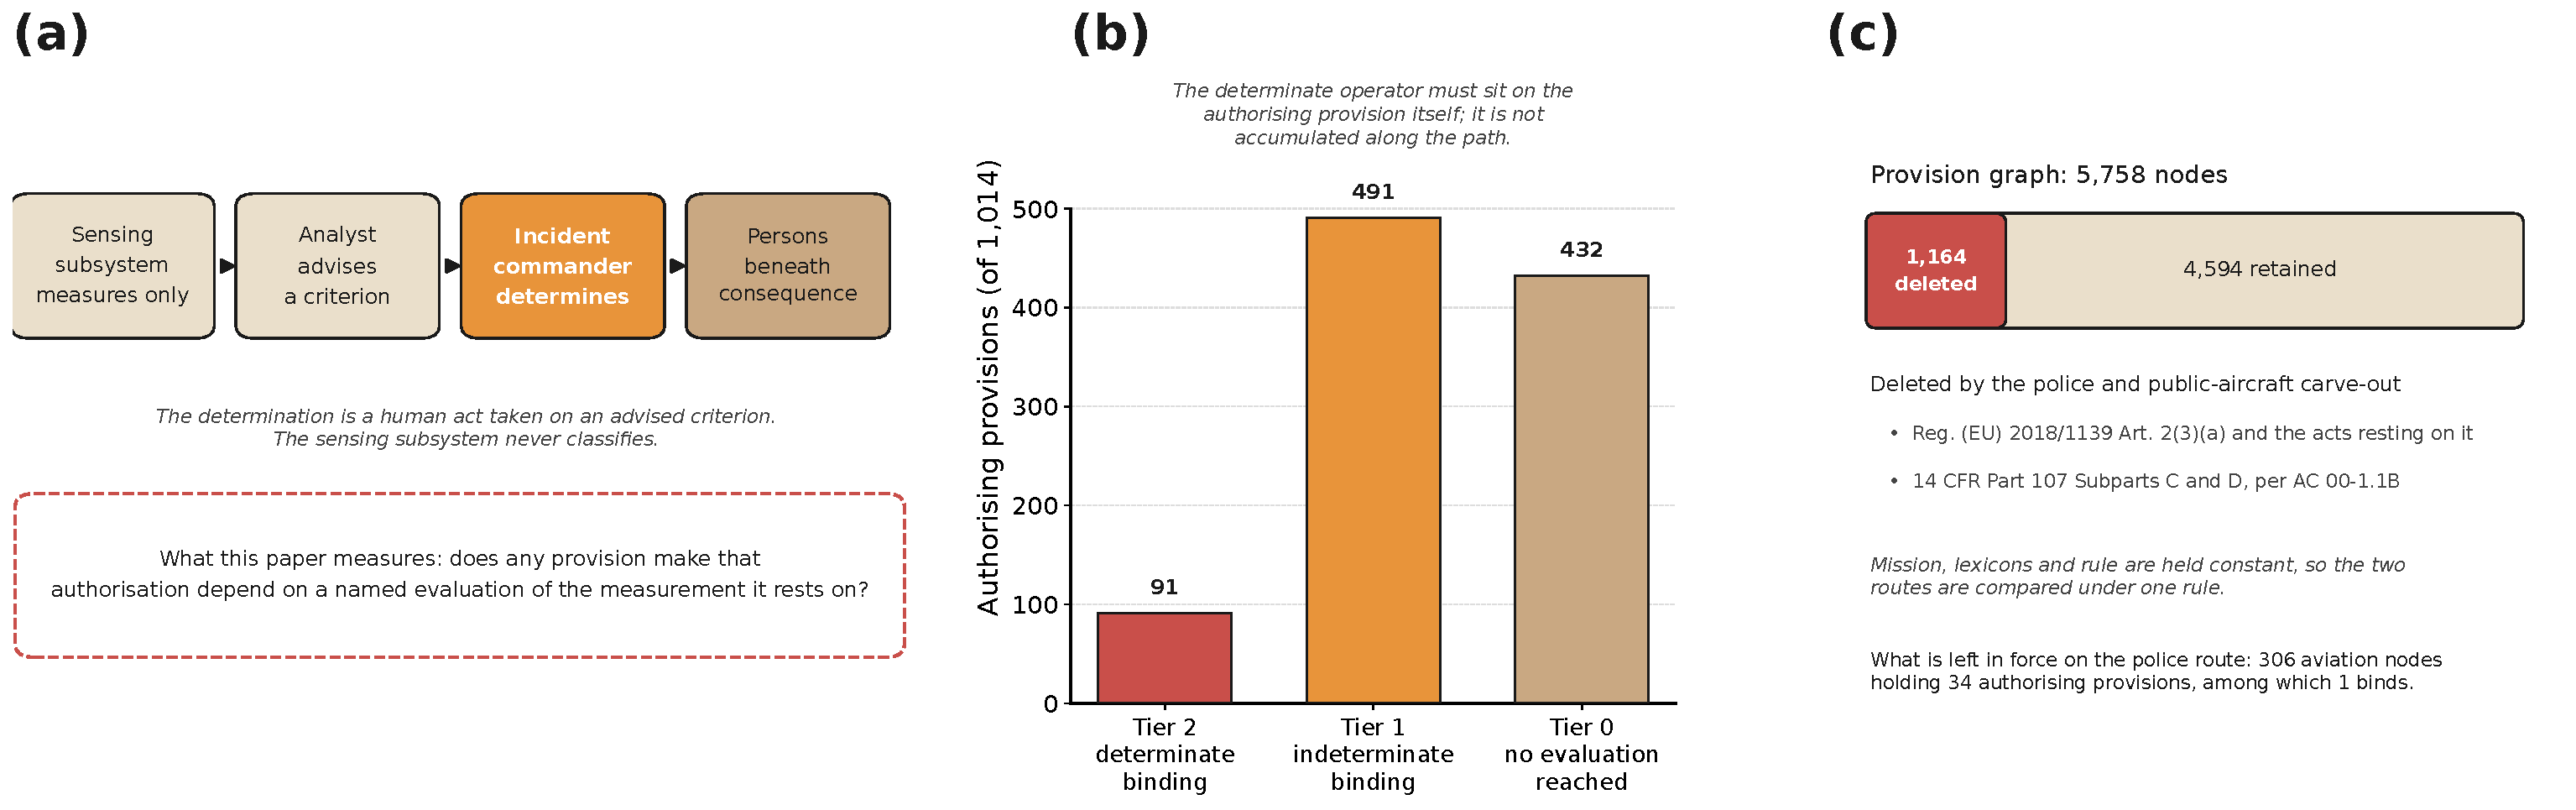
\includegraphics[width=\textwidth]{FigC}
\caption{What is measured. (a) In the ground mission, measurement, analysis and determination are separated by doctrine: the sensing subsystem never classifies, and the determination is a human act taken on an advised criterion. The question this paper measures is whether any provision makes the commander's authorisation depend on a named evaluation of the measurement it rests on. (b) The three tiers an authorising provision can occupy, with the corpus counts. The determinate operator must sit on the authorising provision itself; it is not accumulated along the path. (c) A police and public-aircraft carve-out is implemented as the deletion of nodes from the provision graph, so that the two routes are compared under one rule: Reg. (EU) 2018/1139 Art. 2(3)(a) and the acts resting on it, and 14 CFR Part 107 Subparts C and D per AC 00-1.1B; see Section 3.4 on why that set is conservative. Mission, lexicons and rule are held constant.}
\label{fig:f1}
\end{figure*}

\subsection{The provision graph}\label{sec:2.4}

Each instrument was decomposed to paragraph granularity: an article becomes a hub node carrying its heading, each numbered paragraph a node carrying its own text. Two qualifications on that sentence are owed, because an earlier version of this paper made it without them and it was not true as written. An article with no numbered paragraphs, which in the EU instruments is chiefly a definitions article, carries its numbered definitions instead, each as a node; a definitions article was previously held whole, so a seventeen-thousand-character article counted as one provision and fired on any term anywhere in it. And a United States section with a single unnumbered paragraph was, until the repair reported in Section 2.10, dropped entirely rather than kept as one node. Both are extraction defects and both are reported there with their measured effect. Annexes are cut from the article span and held separately, because EU annexes otherwise merge into the last article of the body. Each annex is held as a single node truncated at 6,000 characters, which is a severe limitation and we state its size: the retained fraction is 3.0\% of Directive 2014/32/EU's annexes, 5.3\% of Regulation 2018/1139's, 7.2\% of 2019/947's, 9.0\% of 2019/945's and 12.9\% of the AI Act's. The instrument-specific maximum permissible error tables of the metrology directive, the class requirements of 2019/945 and Annex III of the AI Act are therefore named in the corpus but not contained in it. A provision that refers to an annex can reach that node, and an evaluation term in the retained opening of an annex will ignite on it, but a condition written into an annex table below the cut cannot be read. Containment edges run downward only, from hub to paragraph and never between siblings, so that an operator in one paragraph is not read as governing its neighbours.

Reference edges were built by jurisdiction-specific grammars operating on paragraph text: EU internal and cross-instrument references; Korean internal references, cross-instrument references by quoted statute name, decree-to-parent-statute references, and the anaphor gateun beop (``the same Act'') resolved against the most recently named statute; Japanese references with kanji-numeral conversion; United States section references within and between Parts 107 and 89; and municipal and state-code internal references. A further two structural edge types were added: chapter and section hubs for the EU instruments, and edges linking a paragraph that says ``this Chapter'', ``this Section'', ``this Regulation'' or ``this Directive'' to the corresponding hub, since such phrases are references without a number.

The graph has 5,758 nodes and 8,834 edges: 4,296 containment, 374 chapter containment, 2,693 numbered internal references, 38 cross-instrument references, 959 unnumbered structural references, 187 decree-to-parent references, 184 annex references and 103 reverse-delegation edges.

\subsection{The predicate}\label{sec:2.5}

Three lexicons operate on node text. eval names a technical evaluation (certification, conformity assessment, test, inspection, audit, impact assessment, verification, accreditation, typeapproval, airworthiness, notified body, declaration of conformity, and Korean and Japanese equivalents). auth names an authorisation outcome (authorisation, permit, licence, registration, approval, placing on the market, eligibility, exemption, and equivalents). det marks determinate conditioning (``shall not . . . unless'', ``only if'', ``shall be revoked'', ``is required to'', and the Korean and Japanese forms that condition a permission on passing an examination), and nondet marks hedges (``should'', bare ``may'', ``as appropriate'', ``where necessary'', and equivalents).

The lexicons carry two exclusions, recorded here because each was introduced to remove a specific false positive. auth excludes activity verbs such as unhaeng and ts\={u}k\={o}; including them

made almost every Korean and Japanese traffic provision an authorisation. det is suppressed where the same unit says that a document must be included with, accompanied by or submitted with an application, because an attachment requirement is a filing formality rather than a condition on the outcome.

A provision is adjudicated as follows. If it carries auth, is not a penalty provision and is a paragraph rather than a hub, it is an authorising provision. From it, a breadth-first search of at most four hops looks for a node carrying eval. The determinate operator must be present on the authorising provision itself; it is not accumulated along the path. If any node on the path carries nondet, the path is capped.

\begin{itemize}
\item Tier 2, determinate binding: the provision carries a determinate operator and reaches a named evaluation within four hops with no hedge on the path.
\item Tier 1, indeterminate binding: the evaluation is reached, but the operator is absent or hedged.
\item Tier 0: no evaluation is reached.
\end{itemize}

The three tiers and the carve-out operation are set out in Fig. 1b and c.

The requirement that the operator sit on the start node is the correction of an error we made. An earlier implementation accumulated it along the path, so a start node with no operator could inherit one four hops away; back-tracing three implausible results exposed it. The uncorrected rule produced a far more striking headline than the corrected one supports, and we state both.

The four-hop bound is not arbitrary. Table 2 reports tier counts as the bound is relaxed. Tier-2 counts saturate: the fifth hop adds 1 return in the whole corpus, and removing the unnumbered structural and chapter edges entirely changes the count by 2.

\begin{table}[!htb]
\centering
\caption{Saturation of the path bound. All conditions use the same 1,014 authorising provisions.}
\label{tab:t2}
\small
\begin{tabular}{@{}lrrr@{}}
\toprule
Condition & Tier 2 & Tier 1 & Tier 0 \\
\midrule
No edges (provision read in isolation) & 72 & 283 & 659 \\
hop $\le$ 1 & 76 & 346 & 592 \\
hop $\le$ 2 & 88 & 442 & 484 \\
hop $\le$ 3 & 90 & 455 & 469 \\
hop $\le$ 4 (adopted) & 91 & 491 & 432 \\
hop $\le$ 5 & 92 & 495 & 427 \\
hop $\le$ 4, structural edges removed & 89 & 489 & 436 \\
\bottomrule
\end{tabular}
\end{table}

\subsection{Validating the lexicon}\label{sec:2.6}

The predicate is only as good as the vocabulary that feeds it, so the vocabulary was tested rather than asserted. The population at risk is tier 1: provisions that authorise and reach an evaluation but were scored as lacking a determinate operator. If the lexicon is leaky, the leak is there.

A sample of 36 tier-1 provisions was drawn with a fixed seed, stratified by language at 12 each for English, Korean and Japanese, and each was read and labelled for whether it does in fact condition an authorisation determinately on a named evaluation. Two of the 36 have since left the authorising population and are excluded. One left under the supplementary-provision repair

described in Section 2.3, having been recorded by the labeller as a transitional provision and not as a false negative. The other, Article 104-2-4(4) of the Japanese Road Traffic Act, was moved into the returned set by the lexicon symmetrisation of Section 2.10 and is therefore no longer in the population at risk; the labeller had recorded it as correctly scored, so its departure does not remove a false negative either. The sample is 34: 12 English, 12 Korean, 10 Japanese. Four were false negatives: 2 of 12 in English, 1 of 12 in Korean, 1 of 10 in Japanese. Allocation was equal across the three strata but the strata are not: the tier-1 population holds 222 English, 120 Korean and 149 Japanese provisions, so a pooled rate that ignores the weights understates the English stratum, which is the one with the highest observed rate. The design-consistent estimate is therefore the stratum-weighted one, 12.6\% with a 95\% interval of [4.7, 29.5] on the logit scale, projecting to 62 missed bindings across the 491 tier-1 provisions with an interval of 23 to 145. The unweighted pooled rate is 11.8\% [4.7, 26.6]; earlier versions of this paper reported that figure, and the weighted estimate replaces it because the sample was stratified and the weights are known.

Two features of this sample bear on that interval and were not stated until a reviewer asked for them. The first is that the sample is clustered by instrument in the same way the corpus is, which is the thing Section 3.3 corrects for elsewhere and did not correct for here. The 12 English provisions come from 6 instruments and both false negatives fall in one of them, the AI Act. The 12 Korean provisions come from 4. The 10 Japanese provisions come from one, the Road Traffic Act, so within that stratum there is no second cluster and the between-instrument component cannot be estimated at all. Treating instruments as sampling units within strata and using t(8) for the 3 strata and 11 instruments widens the interval from [4.7, 29.5] to [2.5, 45.0] per cent, a standard error of 0.083 against the 0.060 the provision-level calculation gives. Dropping the AI Act from the sample moves the weighted rate from 12.6 to 5.1 per cent and the projection from 62 to 25. Both intervals are reported in \texttt{verify/lex\\texttt{\_cluster}.json.} We report the narrower one as the headline because it is the one the stratification was designed for, and we carry the wider one beside it wherever the rate bears weight.

Neither interval is well identified, and the reason is worth stating because it bounds what any single number here can mean. The eight degrees of freedom are the design's, not the data's: one instrument, the AI Act, supplies 69 per cent of the variance, because it is the only sampled instrument in which a false negative occurred more than once. Accounting for that with a Satterthwaite correction gives 6.3 effective degrees of freedom on a per-stratum accounting and 2.0 on a per-instrument one, and the interval runs [2.3, 47.2] or [0.6, 78.2] per cent accordingly. A sample of 34 provisions with four false negatives across 11 instruments does not identify a rate to better than an order of magnitude, which is what this section said at the outset and what the corrected intervals now make arithmetic rather than rhetorical.

The second is that the sample was drawn from a tier-1 population of 480 provisions and the weights are computed on the current population of 491. 16 provisions entered tier 1 between those two states and all 16 are in the Japanese Road Traffic Act, which is 10.7 per cent of the Japanese stratum and had probability zero of being sampled; 5 left, and the two that were in the sample are the two reported above. Calling the estimator design-consistent puts weight on the frame, and the frame is not the population the estimate is about. Re-drawing the sample on the current population would close this and we have not done it.

On interpretation, two points bear. The rate is not higher in the non-English material, which is the asymmetry one would expect if the lexicon were an English instrument applied abroad. And none of the four concerns the sensing or measurement performance of a robot: they are a product conformity assessment on modification, a fundamental-rights impact assessment, a

driver aptitude test and a driving skill test.

Validation found two lexicon defects, and both were repaired before the reported run. The Korean authorisation pattern used a word boundary after the noun, and a word boundary does not occur between two Hangul syllables, so a licence followed directly by a particle did not match. The Korean and Japanese determinacy lists lacked the constructions that condition a permission on passing an examination, which meant the instrument missed Article 85(1) of the Korean Road Traffic Act and Article 89(1) of the Japanese Road Traffic Act, two of the most obvious determinate bindings in the corpus. The Korean construction was added at this stage; the Japanese one was not reached until the lexicon symmetrisation reported in Section 2.10, and Article 89(1) is one of the four Japanese bindings that repair produced.

The labels were applied in a single pass by the same investigator, reading each provision directly rather than through a language model, with no second pass and no second reader. The rate is therefore best read as an order-of-magnitude bound rather than a point estimate, and it is the one place in this paper where a reported figure rests on a single unreplicated reading. The projection it carries into Figure 4c should be read with that in mind.

\subsection{Auditing the bindings}\label{sec:2.7}

The lexicon validation above measures how often the predicate misses a binding. It says nothing about how often what it returns is not one, and that is the population every number in this paper is computed over. We therefore audited it in full rather than by sample.

Each of the 91 provisions the predicate returned was prepared as an audit record containing the provision text, every lexicon pattern that fired on it with the string actually matched and eighty-five characters of surrounding context, the path the predicate recorded, and the node at which an evaluation term ignited. Seventy-three of the 91 were available when the two-pass labelling was carried out. The other 18 entered the returned set afterwards, under corrections reported in Section 2.10: 3 under the operator correction, 5 under the extraction repairs, and 10 under the lexicon symmetrisation. Each of the 18 was prepared as a record in the same form and adjudicated under the same three conditions, by the same procedure but once rather than twice, and the adjudication of each is released with the labels. Every agreement statistic in this section is therefore computed on the 74 records the two passes saw, of which 73 remain in the current returned set, and not on the 91, and a reader who wants the agreement figure for the whole returned set will not find it here, because it was not measured. The 73 records were labelled twice, in two passes carried out by the same investigator using a large language model as the labelling instrument, the second pass made without sight of the first pass's labels and with the records presented in a different order. This is a consistency check on the labelling procedure under repetition, not an inter-rater reliability measurement between two people, and the agreement statistics below should be read only as the former. Both passes applied three conditions derived from the construct itself. A provision is a binding only if (i) it confers or conditions a legal permission, rather than mentioning another regime's permission, defining a term, prohibiting a false mark, deeming a prior authorisation, or listing the documents an application must carry; (ii) the determinate operator conditions that permission, rather than governing a different clause that the pattern window happened to span; and (iii) the object of that condition is a named evaluation procedure, rather than an evaluation term appearing as a date reference, as an item in a definition list, as a section heading, or as the authorisation the provision itself issues.

Labels were recorded on three values, not two: binding, not a binding, and borderline, the third reserved for a record a pass could not place under the conditions as written. The marginals differ between the passes, 43 / 27 / 4 in the first and 26 / 47 / 1 in the second, and the full

\begin{figure*}[!t]
\centering
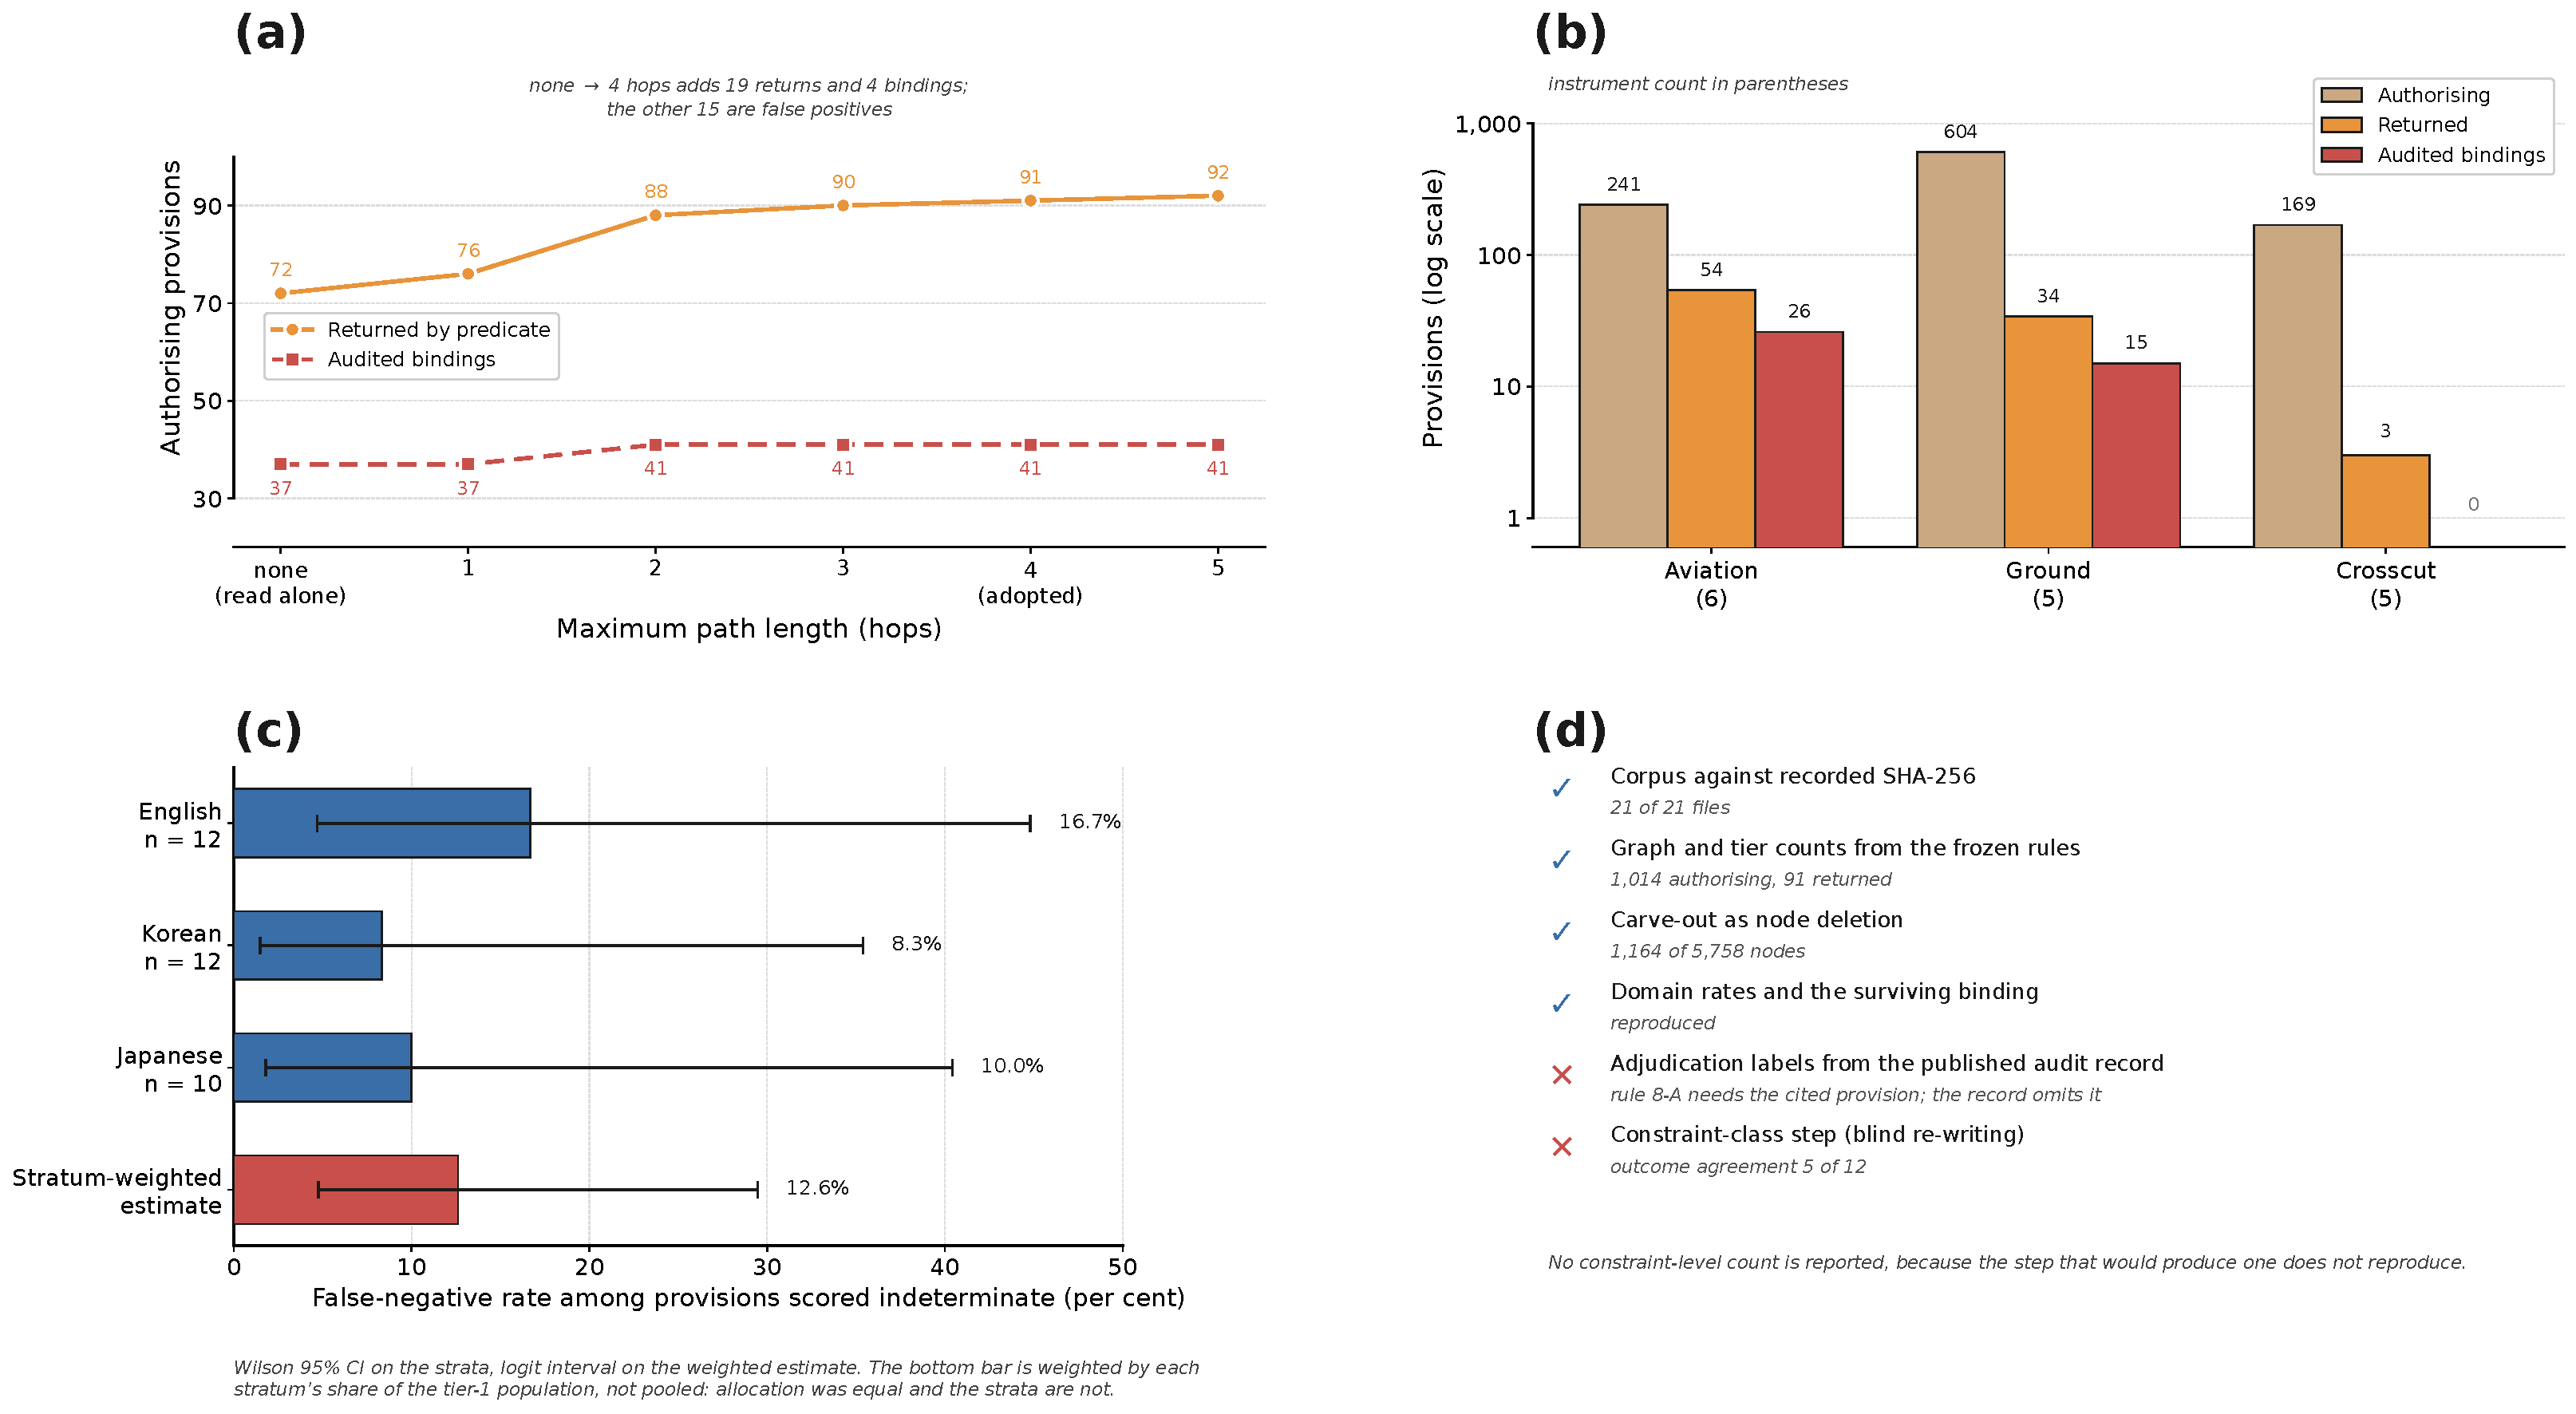
\includegraphics[width=\textwidth]{FigM}
\caption{Checks on the measurement. (a) Provisions the predicate returns and provisions the audit confirms as bindings, both as a function of the maximum path length. Going from a single-provision reading to four hops adds 19 returns and 4 bindings, so the 15 remaining additions are false positives and following cross-references lowers precision from 0.514 to 0.451 (Table 7). (b) Composition of the audited corpus by regulatory domain, with the number of instruments in each. (c) Lexicon validation: the false-negative rate among provisions scored indeterminate, by language, with Wilson 95\% intervals on the strata and a logit interval on the weighted estimate. The plotted interval is the design-consistent one; treating instruments as sampling units within strata widens it to [2.5, 45.0] per cent (Section 2.6). The Japanese stratum is n = 10 because one sampled provision left the authorising population under the repair of Section 2.3 and a second under the symmetrisation of Section 2.10. The bottom bar is the stratum-weighted estimate, not a pooled one: allocation was equal and the strata are not. (d) What reproduces and what does not. The constraint-level step does not, which is why no constraint-level count is reported.}
\label{fig:f2}
\end{figure*}

cross-tabulation is released with the labels, because the three-valued scale is what the agreement statistics below are computed on and a reader who assumes two values will not reproduce them. Agreement between the two passes was 51 of 74, Cohen's $\kappa$ = 0.448. That figure should not be read on the conventional scale, because the two passes have different marginals: 43 / 27 / 4 against 26 / 47 / 1 is a bias index of 0.23, and with those marginals fixed the largest agreement arithmetic allows is 54 of 74, so $\kappa$max = 0.520. The observed $\kappa$ is 86 per cent of its own ceiling. Gwet's AC1, which does not inherit the marginal bias, is 0.577. What the three numbers say together is not that the labelling was moderately reliable but that it was close to as consistent as a systematic shift in threshold between the passes permits. That shift is our own doing: the second pass received an interpretation directive on condition (iii) that the first did not, so the two passes were not given identical instructions, which is why we report agreement both over all 74 labelled records and over the subset that directive does not concern. Eighteen of the twentythree disagreements fall on one sentence pattern, used throughout Regulation (EU) 2018/1139, in which a certificate shall be issued upon application, when the applicant has demonstrated that it complies with the implementing acts of a named article. Restricting to the 56 provisions outside that pattern, agreement is 51 of 56 and $\kappa$ = 0.835. That number estimates nothing. It is obtained by deleting the single cell that holds eighteen of the twenty-three disagreements, so it describes the residue after the disputed pattern is removed and is reported only to locate the disagreement, not to quantify reliability. The disagreement is therefore not instability in the labelling but an ambiguity in condition (iii) that we had not resolved in advance, and we resolve it here, in the direction that excludes: a sentence of that form names no evaluation procedure. The term it offers is either the certificate it is itself issuing, which cannot be its own condition, or the bare verb demonstrated that, which is not a procedure. All eighteen are counted as false positives, as are the three remaining disagreements in which an evaluation term appears only as a descriptor of who is examined or when; the two in which the operator's object is a named examination are counted as bindings.

Forty-one of the 91 provisions are bindings. Precision is 0.451. It is not uniform: 26 of 54 in aviation (0.481), 15 of 34 on the ground (0.441), and 0 of 3 among the cross-cutting instruments (0.000).

The interval on that figure needs saying carefully, because 41 of 91 is a census of the returned set and not a sample from it. The Wilson 95\% interval of [0.352, 0.553] is the interval that would apply if these 91 provisions were a random draw from a larger population of returns. They are not: they are all of them, drawn from sixteen purposively selected instruments, two of which were added late precisely because they were the most likely to refute the paper, and Regulation (EU) 2018/1139 alone supplies 32 of the 91 returns and 17 of the 41 bindings. Resampling the eleven instruments that contribute returns with replacement, 10,000 draws at a fixed seed, and recomputing the precision in each draw, gives [0.306, 0.518], which is a quarter wider and is the interval to use for any statement about how this predicate would behave on instruments other than these sixteen. What that interval generalises over is instruments drawn like these, which is a hypothetical population rather than an observed one, and with eleven clusters it is coarse: the resampled precision takes a limited number of distinct values and the quantiles inherit that discreteness. We report both, and where this paper says that a returned count is an upper bound on bindings, the claim rests on the census point estimate and needs neither interval. Every count this paper reports is therefore given twice, as the number of provisions the frozen predicate returns and as the number that survive the audit, and the second is the one the argument rests on.

This audit establishes the numerator. It says nothing about the denominator, and the denominator was audited separately and found to be contaminated at a comparable rate; Section 2.8

reports that audit and the corrected rates it implies.

The audit names the false positives by mechanism, and one of those mechanisms deserves a paragraph because the obvious repair does not work. The determinate-operator patterns scan a window of up to 200 characters, and the window steps over negation. Article 5(5) of Regulation (EU) 2019/947 says that a UAS operator who has filed a declaration for a standard scenario shall not be required to obtain an operational authorisation, which is an exemption, and the predicate records it as a binding. Nine of the 1,014 authorising provisions carry a determinate pattern inside a negated context and four of those reach tier 2. The repair that suggests itself is to suppress a determinate operator whose match lies within a negated clause. We implemented it and did not adopt it, because it removes a binding as well. Article 5(1) of the same Regulation reads where one of the requirements laid down in Article 4 or in Part A of the Annex is not met, a UAS operator shall be required to obtain an operational authorisation, where the negation governs the condition and the operator is affirmative; a proximity rule cannot tell the two apart, and the paragraph it deletes is the one audited binding that exists only because a cross-reference is followed (Section 3.2). Applied to the corpus the guard returns 88 provisions instead of 91, drops two false positives and one binding, and leaves precision near unchanged at 0.455. Three of the four negated tier-2 provisions fall; the fourth, Article 16(1) of Regulation (EU) 2018/1139, carries a second determinate match outside any negated context and so survives a guard that acts on matches rather than on provisions. Separating the two cases needs the operator's clause boundary rather than a character window, which is the same limit that produces the other mechanisms in this list, so we report the defect and leave the rule alone.

The resolution of condition (iii) was made after the labels were seen, which makes it the one rule in this paper that could have been chosen to suit the answer, so we report what the other choice would have given. Resolving in the direction that includes revives 12 of the records the adjudication rejects and gives 53 bindings instead of 41, a precision of 0.582 instead of 0.451. Every headline survives that change and two of them strengthen: the police carve-out leaves exactly one audited binding in force in either direction (38 to 1 instead of 26 to 1), the cross-cutting instruments still produce none, and the aviation-to-ground ratio rises from 4.34 to 6.35 with Cohen's h from 0.353 to 0.500. We adopt the excluding direction because it is the conservative one on the construct and because it is the direction that makes our own headline weaker, and we report the other so that a reader can see the choice did not manufacture the result (Table 3).

\begin{table}[!htb]
\centering
\caption{Both resolutions of the ambiguity in condition (iii). The adopted direction is the one that yields the smaller count.}
\label{tab:t3}
\small
\begin{tabular}{@{}lrrrrrr@{}}
\toprule
Resolution & Bindings & Precision & Aviation & Ground & Cross-cut & Carve-out \\
\midrule
Excludes (adopted) & 41 & 0.451 & 26/241 & 15/604 & 0/169 & 26 $\rightarrow$ 1 \\
Includes (alternative) & 53 & 0.582 & 38/241 & 15/604 & 0/169 & 38 $\rightarrow$ 1 \\
\bottomrule
\end{tabular}
\end{table}

The audit was performed after the ruleset was frozen and the predicate had been run, and the frozen ruleset was not changed in response to it. Tuning the lexicon or the path bound against these labels would convert a measurement into a fit. The labels, the audit records and the adjudication rule are released with the other materials.

The labels this paper adopts are not the labels its first release reported, and the difference is large enough to state here rather than in a limitation. The two passes described above resolved to 34 bindings, and that is the count the earlier version published. The audit records released with it carried every lexicon match and the path the predicate recorded, but not the text of the provision a path arrived at, so the rule that admits a binding reached through a named provision could not be applied from the record alone; a reader working from the released records could not reproduce the adjudication. We enriched the records with the cited text and had the audit repeated, blind, against a rubric from which the counts had been removed. That pass moves 10 of the 91 records and gives 41. On the binding value the three passes stand at 43, 26 and 41, so the labelling is not stable to the procedure that produces it, and the adopted count is the third pass rather than an average of them. What the change does not move is the comparison the paper rests on: Cohen's h goes from 0.357 to 0.353 and the aviation-against-ground Fisher test from p = 1.5 $\times$ 10$-$6 to p = 2.6 $\times$ 10$-$6 . The direction of the change is against us in the headline rate, which rises from 3.4 to 4.0 per cent, and in favour of us in the precision, which rises from 0.374 to 0.451. All three label sets are released.

\subsection{Auditing the denominator}\label{sec:2.8}

The audit of Section 2.7 establishes that 41 of the 91 provisions the predicate returns are bindings. It leaves the denominator unexamined, and a rate is two numbers. If the authorising population is itself contaminated, every rate in this paper is understated by whatever the contamination is, and the understatement need not be uniform across domains. Reporting a well-audited numerator over an unaudited denominator would be the same error we criticise in the coding literature, one level down.

We therefore audited the denominator by the same procedure. Eighty authorising provisions were drawn with a fixed seed and prepared as records carrying the provision text and the authorisation pattern that fired, with no tier information and no indication of whether the predicate had returned the provision. Each record was labelled against the definition this paper states in Section 2.1: a paragraph of a legal instrument that grants, conditions or withdraws a permission, and is not a penalty provision. As with the binding audit, the records were labelled twice, the second pass in reverse order and without sight of the first. Agreement was 76 of 80. One of the eighty, 14 CFR \S{}89.515, has since left the authorising population under the paragraph-node repair of Section 2.10; the labeller had recorded it as not an authorising provision, so its departure removes a record from the denominator without removing a positive, and the precision below is computed on the 79 that remain. The four disagreements were adjudicated against the provision text: Article 71-5(1) of the Japanese Road Traffic Act, which bars driving without a displayed novice mark, was included because its form is the one this paper counts elsewhere, and three were excluded as procedural duties to issue or record a document, or as a prohibition on using a similar trade name.

Thirty-nine of the 79 remaining sampled provisions authorise: a denominator precision of 0.494 with a Wilson 95\% interval of [0.386, 0.602], projecting the authorising population to 501 provisions with an interval of 392 to 610. The contamination is not uniform, but the pattern is not the one an earlier draw suggested. It is lightest on the ground, where 22 of 40 sampled provisions authorise, and heaviest among the cross-cutting instruments, where 5 of 15 do; aviation falls between at 12 of 24. A first draw, made on the pre-repair population of 1,003, put aviation at 4 of 17 and the pooled precision at 0.375; the two Wilson intervals overlap, but the aviation cell in that draw held four events and we report the second draw rather than the first, because the first was taken over a population two extraction defects have since changed.

The dominant mechanism is institutional and procedural rather than lexical. Of the 41 sampled provisions the audit excludes, the largest groups are duties on an authority or a body to notify, consult, record, verify or issue a document, and provisions allocating tasks, establishing procedures or empowering the Commission to adopt acts. All nine exclusions in the Korean enforcement rule are of this kind, as are six of the nine in Regulation (EU) 2018/1139. Definitions account for three. An earlier draft attributed the contamination chiefly to recitals, definitions and annex headings in the aviation material; that description does not survive the second draw and we withdraw it.

No sampled provision was a penalty provision. The first draw found three that the exclusion patterns missed, all in the Korean and Japanese material; the United States patterns added in Section 2.10 and the second draw together give no further instance, which is evidence that the exclusion now executes, not proof that it is complete.

Table 4 gives the nominal and corrected rates. Correcting the denominator raises the aviation rate from 10.8\% to 21.7\% and the ground rate from 2.5\% to 4.5\%, and because the correction is larger in aviation it widens rather than narrows the contrast the paper rests on: the aviationto-ground ratio goes from 4.3 to 4.8. The corrected rates carry the interval of the denominator

audit, and Table 4 reports them with it; the numerator contributes no interval because the audited binding count is a census of the returned set rather than a sample from it, and an earlier version of this sentence claimed a numerator interval the released script does not compute; the aviation interval runs from 13.9 to 30.4 per cent on a cell of 24 sampled provisions, which is wide enough that we treat the nominal rates as the statement the paper rests on and the corrected rates as a check on their direction. Two further cautions belong with them. The estimator multiplies a nominal count by a sampled precision, so it inherits the upward bias of a plug-in ratio at small cell sizes. And the two draws we have made returned pooled precisions of 0.375 and 0.494; those intervals overlap, but a single point estimate is not a stable basis for correcting a whole population, which is the second reason the nominal pair carries the argument. No conclusion in this paper depends on which pair is used.

\begin{table}[!htb]
\centering
\caption{Binding rates before and after correcting the denominator for the contamination measured in Section 2.8. ``Auth.'' is the nominal authorising count; ``Corr.'' is that count multiplied by the audited precision of the denominator in that domain, and the interval on the corrected rate carries the Wilson interval of that precision. The audited binding count is the same in both columns, because the binding audit's condition (i) applies the same test as the denominator definition, so a provision counted as a binding is by construction inside the true authorising set. The corrected figures rest on domain cells of 24, 40 and 15 sampled provisions and should be read with that in mind; the plug-in estimator B/(N $\hat{p}$) is also upward-biased at these cell sizes. The Wilson intervals in this table are computed on provisions and carry no correction for the instrument clustering that Section 3.3 measures; the corrected intervals of Table 9 are the ones that carry it. The corrected authorising counts do not add: the three domain cells sum to 508 against the 501 in the Total row, because the plug-in estimator is applied to each cell's own audited precision and is not additive across cells.}
\label{tab:t4}
\small
\begin{tabular}{@{}lrrrrrr@{}}
\toprule
Domain & Bindings & Auth. & Nominal & Denom. prec. & Corr. auth. & Corrected rate \\
\midrule
Aviation & 26 & 241 & 10.8\% & 12/24 = 0.500 & 120 & 21.7\% [15.7, 34.3] \\
Ground & 15 & 604 & 2.5\% & 22/40 = 0.550 & 332 & 4.5\% [3.6, 6.2] \\
Cross-cut & 0 & 169 & 0.0\% & 5/15 = 0.333 & 56 & 0.0\% \\
Total & 41 & 1,014 & 4.0\% & 39/79 = 0.494 & 501 & 8.2\% [6.7, 10.5] \\
\bottomrule
\end{tabular}
\end{table}

\subsection{The carve-out as node deletion}\label{sec:2.9}

Mission A can be flown on two routes. The civil route is adjudicated against the full corpus; the police route against the same corpus with the provisions that do not apply to police operations deleted from the graph. Everything else is held constant, so the difference between the two is a measurement rather than an argument.

Deletion is driven by two documented carve-outs. Regulation (EU) 2018/1139 Article 2(3)(a) provides that the Regulation does not apply to aircraft, and equipment to control aircraft remotely, while carrying out military, customs, police and similar activities or services under the control and responsibility of a Member State, undertaken in the public interest by or on behalf of a body vested with the powers of a public authority, together with the personnel and organisations involved; Regulations (EU) 2019/947 and 2019/945 rest on that basic act and are deleted with it.

Three features of that provision bear on what the deletion models, and we state them because the first two narrow it and the third is the reason the comparison is worth making at all. The exclusion is indexed to an activity rather than to an airframe: while carrying out means that the same unmanned aircraft is inside the Regulation on Monday and outside it on Tuesday, according to what it is doing. The deletion therefore models a specific condition, a police mission flown under the control and responsibility of a Member State by a body vested with public-authority powers, and not a standing status that attaches to police equipment. It also carries conditions of

its own that a real agency would have to satisfy, and an operation failing any of them stays inside the Regulation.

The third is that the exclusion is not a void. The second subparagraph of Article 2(3) provides that Member States shall ensure that the activities and services performed by those aircraft are carried out with due regard to the safety objectives of this Regulation, and that where appropriate those aircraft are safely separated from other aircraft. That is the whole of what survives the carve-out on the European side, and its two operative standards are due regard and where appropriate, both of which this paper's own hedge lexicon matches. The provision that replaces a certification regime for police flight is, on the predicate's own reading, indeterminate. We report this as a legal reading of the carve-out rather than as a measurement, because Article 2(3) is a scope provision and the audited population is drawn from authorising provisions; the predicate does return it, at tier 1. FAA AC 00-1.1B paragraph 12 states that other civil certification and safety oversight regulations do not apply to public aircraft operations, and that a public aircraft operator may self-certify standards for unmanned aircraft airworthiness as well as pilot certification, qualification and medical standards; 14 CFR Part 107 Subpart C and Subpart D are deleted accordingly.

This removes 1,164 of 5,758 nodes: 682 from Regulation 2018/1139, 232 from 2019/945, 133 from 2019/947, 68 from Part 107 Subpart C and 49 from Subpart D. Subparts A, B and E of Part 107 are retained, as is the whole of Part 89, which is not among the provisions AC 00-1.1B exempts. Every borderline case was resolved in favour of retention, which is the direction that makes the police route look better covered than it is.

Deleting Regulation 2019/945 needs its own justification, because that Regulation imposes duties on a manufacturer placing a product on the market rather than on the operator who later flies it, and an operator-side exemption does not obviously reach it. The justification is in its own scope provision. Article 2(1) states that Chapter II applies to UAS intended to be operated under the rules and conditions applicable to the `open' category of UAS operations or to operational declarations under the `specific' category of UAS operations pursuant to Regulation (EU) 2019/947. The class-marking regime is therefore indexed to operation under 2019/947, which is the regime the police route does not enter. We none the less report what happens if the objection is granted, because the answer does not depend on resolving it: retaining the whole of Regulation 2019/945 on the police route raises the returned count from 7 to 8 and leaves the audited count at 1, the same surviving binding. Regulation 2019/945 contributes no audited binding on either route, so its treatment cannot change the result (Table 5).

The second variant is the one that does change it. Article 2(6) of Regulation 2018/1139 allows a Member State to decide to apply parts of Chapter III to the activities excluded by Article 2(3)(a). No such decision is modelled in the adopted deletion, which is why the Limitations call the carveout elective rather than automatic. Restoring the whole of Regulation 2018/1139 puts 18 audited bindings back in force on the police route, 17 of the 25 audited bindings the carve-out removes. We previously called this an upper bound on what such a decision could return; it is not one. Section VII of Chapter III is Unmanned aircraft, and Implementing Regulation 2019/947 and Delegated Regulation 2019/945 are adopted under it, so a Member State decision applying that Section would plausibly carry those acts with it, and this row restores only the basic act. It is a partial restoration and the figure is a lower bound on what the decision could return, not an upper one.

\begin{table}[!htb]
\centering
\caption{The police route under three deletion sets. The adopted set is the first row. The second grants the objection that the product regime is not operator-indexed; the third is a lower bound on a Member State decision under Article 2(6).}
\label{tab:t5}
\footnotesize
\begin{tabularx}{\textwidth}{@{}Xrrr@{}}
\toprule
Deletion set & Nodes retained & Returned & Audited \\
\midrule
Adopted & 4,594 & 7 & 1 \\
Regulation 2019/945 retained & 4,826 & 8 & 1 \\
and 2018/1139 also restored (Art. 2(6), partial) & 5,508 & 40 & 18 \\
\bottomrule
\end{tabularx}
\end{table}

\subsection{Freezing and falsification}\label{sec:2.10}

Seventy-nine files are frozen: the corpus manifest and the provision graph, the lexicons, the node extractor, the reference grammars, the structural-edge builder, the path and tier logic, the scope restriction, the carve-out rule, the adjudication executor and its label register, the three label files, every script that writes an output this paper cites, the script that assembles this manuscript from its parts, and the four figure scripts with the eight image files they produce, and the script that measures how saturated the evidence vocabulary is. The files are hashed individually and the concatenation of their hashes is hashed again. The count in the preceding sentence is the one \texttt{verify/seal\\texttt{\_audit}.py} prints, and a released check fails if the two differ; an earlier version stated forty-five while the register held forty-seven, in the same paragraph that had just assigned the count to the script.

An earlier version of this sentence said that every file which can influence an outcome was frozen, and a reviewer established that it was not true. The scope restriction, which is the sole source of the domain partition and whose admissibility test the frozen adjudication executor imports, was outside the seal, as was the adjudication label register that produces the audited count itself. Ten modules present in the first freeze had been dropped without record by the time of the fourteenth, and twenty-five of the scripts that write cited outputs were never in it, one of them a script the freeze record itself names as affecting measurement. All are now inside. We no longer state the seal as exhaustive: a released script, \texttt{verify/seal\\texttt{\_audit}.py}, counts what it does not cover on every run and fails if any script that writes a cited output sits outside it, and the count it reports is the claim rather than our assertion.

Two further gaps in the apparatus were found after that and are closed here rather than disclosed. The first is that the apparatus sat outside the thing it audits: the script that computes the generation hash was not itself among the frozen files, so replacing its output with a constant left every gate passing. Eleven files of apparatus, the hash script and the four gates that read it among them, are now frozen with the rest. The three files that hold the consistency suite were outside the seal until this version, which mattered because a check can be replaced by a trivially true one without changing the number of checks the suite reports; those three are frozen as well, so a change to any of them moves the generation hash.

A third gap was of the same kind and was created by one of these repairs. The check that the figures in the manuscript are the ones the released figure scripts produce compared each figure against a record of hashes, and that record was written by the build script, which the gate runner invokes immediately before the check. The build script does not regenerate the figures; it copies them. So the record was always a record of whatever was on disk at that moment, and the check could not fail. We established the size of this by replacing one results figure with another of the paper's own figures: every gate and every check passed. The expected hashes now come from the freeze record, which only an explicit refreeze writes, and the figure scripts and their outputs are in the seal, so a substitution moves the generation hash as well. The same repair removed a

comment that claimed the assembled manuscript was checked by reassembling it and comparing bytes while the code compared hashes the build had just written; the assembly logic is now a separate released script and the check reassembles with it and compares bytes, which does not depend on what ran first.

That does not close the hole, and saying that it did would repeat the error. A reviewer put it back in three lines: replacing the hash function's output with a constant and then altering a frozen input still leaves every gate passing, because the hash that is supposed to detect the alteration is computed by a file the alteration can reach. Sealing the apparatus inside its own seal is circular. What actually caught the substitution was the consistency suite comparing each frozen file against the per-file digests recorded in the freeze record, and the freeze record is not in the seal. So the root of the guarantee is one file outside the thing it guarantees, and anyone who can write that file can write a consistent set. We state the position rather than a stronger one: the apparatus detects accident and drift, which is what it was built for and what it has repeatedly done, and it does not detect an author who edits both an input and the record of that input. The only fix is an external anchor, and the deposited archive's identifier is where the freeze record's hash is pinned beyond our reach; until that identifier exists, the chain is internal and we do not claim otherwise. The second is the provenance stamp each output carries. It was written afterwards by a separate pass that selected files by modification time, which could be reproduced with two shell commands and which, on the same frozen inputs, stamped a different set of files on each run. Each script now writes its own stamp at the moment it writes its output, and the stamping pass is retired. The stamp therefore records that this generation's code produced this output. It is not evidence that nothing was altered afterwards, because whoever can write the output can write the stamp, and we do not offer it as such. Two outputs were also exempt from the freshness gate on the stated ground that they were corpus facts independent of the ruleset. That ground was wrong, since the corpus manifest and the node extractor are both frozen, and while the exemption held, one of the two came to hold an annex length that the current corpus does not reproduce. Both are now regenerated and checked with the rest. The adjudication re-runs bit-identically across hash seeds, which required sorting the adjacency lists; an earlier version reported tier counts stably but recorded paths that varied between runs, and the claim of bit-identical reproduction was not true until this was fixed.

Ten changes have been made to the frozen files and rules since, and each is recorded with its measured effect rather than absorbed silently. Appendix A gives them in full, one paragraph each, with what prompted the change and what it moved. Table 6 gives the net effect of the set on the quantities this paper reports, so that a reader who wants to know whether the ruleset was tuned to the answer can see the direction of every move without reading the appendix. Three of the ten moved a headline figure against us, four moved one in our favour, and three left every reported quantity unchanged; the two largest in absolute terms are the lexicon symmetrisation, which added nine returned provisions and four audited bindings, and the paragraph test, which removed five authorising provisions from the aviation denominator and so raised the aviation rate.

Nothing else was altered: no path bound, hedge rule or scope restriction was changed in response to the audit, although the audit identifies several that would raise precision if changed. All ten are reported because a frozen ruleset is only worth freezing if departures from it are visible, and the hash chain of the current files is republished with the materials so that the versions can be compared.

The design states its own defeater, and the defeater was met. The claim an earlier version of this paper made was that outside aviation, and inside aviation outside the civil route, no provision

\begin{table}[!htb]
\centering
\caption{Net measured effect of the ten changes to the frozen files and rules. ``Before'' is the state at the first freeze that reported each quantity, and for the rows that depend on labels it is that state as labelled then, because the pre-change returned sets were not re-labelled under the adjudication this paper adopts; ``after'' is the current frozen run. Appendix A attributes each move to the change that produced it. Direction is relative to the claim this paper makes: a change that raises the predicate's precision, or lowers the rate at which bindings appear, makes the paper's negative claim easier to sustain and is marked favourable.}
\label{tab:t6}
\small
\begin{tabular}{@{}lrrr@{}}
\toprule
Quantity & Before & After & Direction \\
\midrule
Corpus nodes & 5,568 & 5,758 & neutral \\
Graph edges & 8,596 & 8,834 & neutral \\
Authorising provisions & 1,003 & 1,014 & neutral \\
Returned provisions & 77 & 91 & against \\
Audited bindings & 27 & 41 & against \\
Precision of the predicate & 0.351 & 0.451 & favourable \\
Aviation-to-ground ratio & 8.07 & 4.34 & against \\
Lexicon false-negative rate & 11.1\% & 12.6\% & against \\
Surviving binding on police route & 1 & 1 & unchanged \\
\bottomrule
\end{tabular}
\end{table}

conditions a determinate authorisation outcome on a named evaluation of a performance property of the machine; one provision that authorises, carries a determinate operator and reaches such an evaluation within four hops would refute it. Section 3.4 reports that provision. It is 14 CFR \S{}89.110(b), it survives the police carve-out, and it is the reason the claim this paper now makes is narrower and is stated in terms of what the evaluation is about. The surviving binding conditions operation on an accepted declaration that the aircraft reports its own position to a stated accuracy. It says nothing about the accuracy of anything the aircraft senses, and the corpus contains no provision in force on the police route that does. This is a weaker claim than the one we set out to test and it is the one the measurement supports. The corpus, graph, lexicons and executor are released so that the search can be run by anyone, including against instruments we did not include, and the defeater stands in the same form: one provision in force on the police route that conditions an authorisation on a named evaluation of sensing performance refutes it.

\section{Results}\label{sec:3}

\subsection{Thirty-four of 1,014 authorising provisions are determinate bindings}\label{sec:3.1}

Across the corpus, 1,014 provisions authorise. The frozen predicate returns 91 of them as determinate bindings; 491 reach an evaluation without a determinate operator; and 432 reach none. The audit of Section 2.7 then separates the 91: 41 are bindings and 50 are not, a precision of 0.451; this is a census of the returned set, with a Wilson 95\% interval of [0.352, 0.553] and an instrument-clustered bootstrap interval of [0.306, 0.518] (Section 2.7).

Determinate binding is therefore the exception twice over. It is the exception among authorising provisions, at 4.0\% of the 1,014 after audit against 9.0\% before it, and the indeterminate case is the mode by an order of magnitude. And it is the exception among the provisions the predicate itself returns, nearly two thirds of which do not withstand reading. Both of those denominators are themselves audited: Section 2.8 measures the authorising population to be contaminated at 0.494, which raises the corpus-wide rate from 4.0\% to 8.2\% and raises it unevenly, so the rate is reported in both coordinates wherever it carries an argument.

Both numbers are reported throughout. The first states what a frozen, published rule returns and can be reproduced from the released files without reading a word of law; the second states what survives a reader, and is the number every substantive claim below rests on. Where they

differ the difference is reported, because the gap between them is itself a finding about what automated regulatory measurement can and cannot assert.

\subsection{Following cross-references does not reveal hidden bindings}\label{sec:3.2}

The central methodological claim of this design is that a binding is a property of a path rather than of a provision, and that reading provisions one at a time therefore understates how much technical binding a corpus contains. The audit allows that claim to be tested rather than asserted, because it separates the bindings the predicate finds into those that survive reading and those that do not. It does not survive the test.

Deleting every edge and asking only what each paragraph says on its own returns 72 provisions that satisfy the predicate. Thirty of them are audited bindings. Restoring the cross-reference graph raises the count to 91 and the audited bindings to 34. The graph therefore contributes four additional bindings and fifteen additional false positives (Table 7). Of the 41 audited bindings, 37 (90.2\%) are visible in a single paragraph read alone, and 4 (11.8\%) exist only because a reference is followed. The conclusion is unchanged in direction and weaker in degree: precision still falls monotonically as the bound is relaxed, from 0.417 on a single-paragraph reading to 0.451 at four hops, so following cross-references still costs more in false positives than it buys in bindings.

\begin{table}[!htb]
\centering
\caption{What the cross-reference graph adds. Each row applies the frozen predicate at a different path bound to the same 1,014 authorising provisions; the audit of Section 2.7 then separates the provisions it returns. Precision falls monotonically as the bound is relaxed.}
\label{tab:t7}
\small
\begin{tabular}{@{}lrrrr@{}}
\toprule
Condition & Audited bindings & False positives & Returned & Precision \\
\midrule
No edges (provision read alone) & 37 & 35 & 72 & 0.514 \\
hop $\le$ 1 & 37 & 39 & 76 & 0.487 \\
hop $\le$ 2 & 41 & 47 & 88 & 0.466 \\
hop $\le$ 3 & 41 & 49 & 90 & 0.456 \\
hop $\le$ 4 (adopted) & 41 & 50 & 91 & 0.451 \\
\bottomrule
\end{tabular}
\end{table}

The single binding that the graph does contribute is the one the design was built to catch. Article 5(1) of Regulation (EU) 2019/947 requires a UAS operator to obtain an operational authorisation pursuant to Article 12 where a requirement of Article 4 or Annex Part A is not met, and Article 12(1) is where the competent authority shall evaluate the risk assessment and the robustness of the proposed mitigating measures. The operator, the referral and the evaluation are written in three places, and only following the reference assembles them. That this structure exists is not in doubt. What the audit shows is that it is rare, and that the same traversal which finds it also manufactures 15 returns that are not bindings.

This runs against our own earlier reporting, and we state the correction plainly. An earlier, unsubmitted draft of this manuscript reported that 19 of 78 bindings, a quarter of the total, were invisible to provision-by-provision reading, and drew from that the methodological conclusion that provision-level audits systematically understate the hardest category. That figure was computed over unaudited counts. Once the counts are audited it inverts: the provisions that the graph adds are overwhelmingly provisions in which an authorisation and an evaluation word happen to lie within four hops of one another without the second conditioning the first. For this corpus, reading each authorising provision on its own is not a weaker instrument than following its references. It is a more precise one.

Two qualifications bound that conclusion. It is a statement about precision, not about recall: the audit samples only provisions the predicate returned, so it cannot say how many bindings a single-provision reading would miss, and the lexicon validation of Section 2.6 bears on that question instead. And it is a statement about this corpus, in which cross-references between a determinate operator and a named evaluation turn out to be uncommon; a corpus of framework statutes that delegate their technical content wholesale would not behave this way.

\subsection{What binds is the machine, and the pooled ground rate hides it}\label{sec:3.3}

The 41 audited bindings are not spread evenly across regulatory domains (Table 9). Aviation instruments convert 10.8\% of their authorising provisions into audited bindings. Ground-robot and road-traffic instruments convert 2.5\%. The cross-cutting instruments that govern data protection, artificial intelligence, measuring instruments and police equipment convert none at all. The aviation-to-ground ratio is 4.34, with Cohen's h = 0.353. Correcting both denominators for the contamination measured in Section 2.8 raises the two rates to 21.7\% and 4.5\% and the ratio to 4.8, because the contamination is heavier in aviation; the nominal pair is the conservative statement of the contrast and is the one quoted throughout.

Wilson 95\% intervals on the three nominal rates are [7.5, 15.3], [1.5, 4.1] and [0.0, 2.2] per cent, and those intervals assume provisions are independent. They are not, for the reason given next, and under the design effect measured there they widen to [4.9, 22.1], [0.9, 6.8] and [0.0, 9.6]. Both are reported in Table 9 and the wider pair is the one any comparison between domains has to use.

The unit of analysis is the instrument, not the provision. Earlier versions of this paper tested this contrast with a Fisher exact test over provisions and reported p = 1.5 $\times$ 10$-$6 with an odds ratio of 5.7. That test is withdrawn as a finding, and the reason is visible in the data it was run on. Bindings do not arise independently provision by provision; they arise where an instrument is drafted to condition permissions on technical evaluation, and then they arise in numbers inside that instrument. Of the 26 aviation bindings, 24 are in two instruments, 17 in Regulation (EU) 2018/1139 and 7 in 14 CFR Part 107, and two of the six aviation instruments contribute none. All 15 ground bindings are in four of the five ground instruments. The intraclass correlation of the binding indicator across the sixteen instruments is 0.067, which at an effective (Kish) cluster size of 56 provisions, against an arithmetic mean of 63 and a median of 34, gives a design effect of 4.68 and an effective sample size of 217 against a nominal 1,014. A provision-level test on this structure counts each instrument's drafting decision once per provision, which is pseudoreplication, and it is the error this paper is otherwise about.

Taking the instrument as the unit, the contrast does not reach conventional significance and we say so plainly. There are six aviation instruments and five ground instruments. Relabelling them across the two domains gives 462 partitions, and the observed difference in pooled rates is equalled or exceeded in 41 of them: p = 0.09. A Mann-Whitney test on the eleven instrumentlevel rates gives p = 0.52. A design-effect correction applied to the provision-level table gives p = 0.018, but that correction treats the design effect as if it were a known constant and we do not rest on it. With six instruments against five, no test on this corpus has the power to separate the domains; the corpus is too small in its own unit of analysis, and that is a property of the available law rather than of the measurement.

What survives is therefore descriptive and we state it as such. Aviation instruments carry audited bindings at about five times the rate of ground instruments, the direction is the same in every instrument-level comparison, and the concentration in Regulation (EU) 2018/1139 and

Part 107 is the substantive observation: the contrast is between drafting traditions of particular instruments, not between two populations of provisions that a test could separate. Cohen's h = 0.353 sits in the range conventionally read as a small effect, and that is consistent with a large ratio between two small proportions, which is what h is designed to discount. Both effect measures carry intervals and we give them, because a ratio reported without one invites the reading the previous sentence warns against. On provision-level standard errors the ratio runs [2.34, 8.06] and h runs [0.20, 0.50]; under the design effect of 4.68 they run [1.14, 16.53] and [0.03, 0.68]. The corrected interval on the ratio excludes 1, and an earlier version of this paragraph called that the one inferential statement about domains this corpus supports. It is not, and the reason is the one the paragraph above gives for setting the corrected Fisher test aside: both treat the design effect as a known constant when it is estimated from the 16 instruments of the corpus. Held to that standard the interval does not survive. The design effect at which the lower bound reaches 1 is 5.65 against the 4.68 measured, so a 21 per cent movement in the design effect removes the exclusion. Dropping any one of four instruments (Regulation 2018/1139, 14 CFR Part 107, the Japanese Road Traffic Act, the Korean Road Traffic Act Enforcement Rule) removes it outright. Resampling with replacement the 11 instruments that contribute to the ratio, and recomputing the design effect in each draw, the corrected interval includes 1 in 53 per cent of the 9,864 draws in which the ratio is defined (136 of 10,000 draws lose one domain's bindings entirely and are discarded), with the design effect itself running [1.00, 8.23], where 955 draws return a negative variance-component estimate and are floored at 1. An earlier version resampled all sixteen instruments, including the five that contribute nothing to the ratio, and reported 54 per cent of 10,000; the figure here is both the one the released script computes and the less favourable of the two. We therefore make no inferential claim about domains. What the corpus supports is the ordering and the census, and a reader who concludes from the ratio that aviation law densely conditions authorisation on technical evaluation has read more into it than the figure carries.

The carve-out comparison in Section 3.4 is not affected by any of this. It is a census of one population of provisions under two bodies of law, with the corpus, the predicate and the labels held constant, so it requires no test and no independence assumption; what it reports is what the deletion removes, not an inference from a sample.

That is as far as the pre-registered partition goes, and it is not far enough, because the ground category is not one body of law. Of its 604 authorising provisions, 574 are road-traffic instruments that regulate human drivers and only 30 are the Korean robot instruments. Those two have no reason to behave alike, and they do not. We therefore repartitioned the same 41 audited bindings by subject matter, after seeing the composition of the ground corpus and before writing this paragraph, and report it as the post-hoc analysis it is (Table 8).

This partition is subject to the same objection as the pre-registered one, and for the same reason: its cells are instruments, and provisions inside an instrument are not exchangeable. We therefore report it descriptively and give the provision-level tests only as the quantity a reader would otherwise compute, labelled as what they are. Aviation certification carries bindings at a higher rate than road-traffic law, 26 of 241 against 14 of 574, and a provision-level Fisher exact test on that table gives p = 2.6 $\times$ 10$-$6 with an odds ratio of 4.8; against horizontal product law, 26 of 241 against 0 of 139, it gives p = 6.7 $\times$ 10$-$6 , and against the pooled cross-cutting denominator p = 9.3 $\times$ 10$-$7 . None of these is offered as a tested finding. Each is computed over provisions, the design effect of the instrument clustering is 4.68, and the two aviation bindings outside Regulation (EU) 2018/1139 and Part 107 are what any instrument-level test would have to work with.

An earlier version of this paper declined one of these comparisons on the ground that a cell holding no events carries no test, while performing another that pools the same cell with a smaller

\begin{table}[!htb]
\centering
\caption{The same 41 audited bindings repartitioned by subject matter. This partition is post-hoc: it was made after the composition of the ground corpus was seen, and it is reported because the pre-registered partition pools instruments that do not behave alike. Rates are audited bindings over authorising provisions, with Wilson 95\% intervals. The instrument counts in parentheses are: aviation certification is Regulations 2018/1139, 2019/947 and 2019/945, 14 CFR Parts 107 and 89 and AC 00-1.1B; robot certification is the Korean intelligent robots act and its decree; road traffic is the Japanese and Korean road traffic instruments; police conduct is the Law Enforcement Directive, the Seattle ordinance and the California code; horizontal product law is the AI Act and the Measuring Instruments Directive.}
\label{tab:t8}
\small
\begin{tabular}{@{}lrrrrr@{}}
\toprule
Subject & Auth. & Audited & Rate & Wilson 95\% CI & Design-effect 95\% CI \\
\midrule
Aviation certification (6) & 241 & 26 & 10.8\% & [7.5, 15.3] & [4.9, 22.1] \\
Robot certification (2) & 30 & 1 & 3.3\% & [0.6, 16.7] & [0.2, 41.5] \\
Road traffic, drivers (3) & 574 & 14 & 2.4\% & [1.5, 4.1] & [0.8, 6.9] \\
Police conduct (3) & 30 & 0 & 0.0\% & [0.0, 11.4] & [0.0, 37.5] \\
Horizontal product law (2) & 139 & 0 & 0.0\% & [0.0, 2.7] & [0.0, 11.5] \\
\bottomrule
\end{tabular}
\end{table}

one. The stated criterion was wrong: power depends on the denominator rather than on the count in the empty cell, and applying it inconsistently withheld a quantity while reporting its pooled cousin. We correct it here, and the correction promotes nothing, because the unit of analysis defeats every number in this table equally. The small-cell comparisons show the same thing from the other end. Robot certification returns 2 of 30, with a Wilson interval of [1.8, 21.3] per cent wide enough to contain both the aviation and the road-traffic rate, so the failure of a provision-level Fisher test to separate it from aviation (p = 1.00) is an absence of power and not a finding of equivalence. The police-conduct instruments return 0 of 30 and are not separable from the aviation rate either (p = 0.088).

The two zero cells deserve a sentence of their own, because the design effect changes what they support. On provision-level Wilson intervals, horizontal product law at 0 of 139 has an upper bound of 2.7 per cent, which sits below the aviation rate of 10.8 per cent, and the crosscutting denominator at 0 of 169 has an upper bound of 2.2 per cent; read that way, each excludes the aviation rate. Under the design effect of 4.68 the bounds move to 11.5 and 9.6 per cent and neither excludes it. We had leaned on the first of these as the quantitative support for treating horizontal product law as a different regime from aviation certification, and on the corrected interval it does not carry that weight. What the table supports is an ordering of instruments by rate, with the two densest instruments identified, and not a claim that the categories differ.

What the repartition establishes is therefore negative and it is about our own pre-registered partition rather than about the law. The pooled ground rate of 2.5\% is produced by a denominator that is 95\% human driver licensing, so it cannot be read as a statement about ground robotics, and the pooled cross-cutting zero is carried by the AI Act and the metrology Directive, which supply 139 of the 169 provisions while the instruments that actually regulate police conduct supply 30. Both pooled figures appear in Table 9 and in our earlier drafting, and both should be read as descriptions of a mixed denominator. The statements this paper rests on about police-conduct instruments and about the Korean robot statute are readings of their text, set out in Sections 4.4 and 3.4, not statistical contrasts.

The objects the aviation bindings attach to are worth stating precisely, and we measured them rather than asserting them. Each of the 41 audited bindings was classified, in two passes over its own text carried out the same way as the binding audit of Section 2.7 and subject to the same caveat, by which permission it conditions: permission to supply the artefact (design, produce, type-certify, place on the market) or permission to operate it (fly, drive, conduct an operation,

\begin{table}[!htb]
\centering
\caption{Bindings by regulatory domain, before and after audit. No analyst-written search terms enter the returned column; it is computed from the lexicons and the graph over all authorising provisions. The audited column applies the labels of Section 2.7. Precision differs by a factor of nearly two between aviation and the ground corpus and is zero across the cross-cutting instruments, so the returned counts are not comparable between domains and the audited counts are. Aviation is Regulations 2018/1139, 2019/947 and 2019/945, 14 CFR Parts 107 and 89, and AC 00-1.1B; ground is the Japanese and Korean road traffic instruments and the Korean intelligent robots instruments; cross-cutting is the AI Act, the Measuring Instruments Directive, the Law Enforcement Directive, the Seattle ordinance and the California code.}
\label{tab:t9}
\small
\begin{tabular}{@{}lrrrrrr@{}}
\toprule
Domain & Auth. & Ret. & Aud. & Rate & Design-effect 95\% CI & Precision \\
\midrule
Aviation (6 instruments) & 241 & 54 & 26 & 10.8\% & [4.9, 22.1] & 0.481 \\
Ground (5 instruments) & 604 & 34 & 15 & 2.5\% & [0.9, 6.8] & 0.441 \\
Cross-cutting (5 instruments) & 169 & 3 & 0 & 0.0\% & [0.0, 9.6] & 0.000 \\
Total & 1,014 & 91 & 41 & 4.0\% &  & 0.451 \\
\bottomrule
\end{tabular}
\end{table}

use a facility). The passes agreed on all 41, including on the single provision each recorded as borderline; as there, the figure measures repeatability of a procedure, not agreement between two readers. The borderline record was resolved against the provision text by the procedure of Section 2.7.

Thirty-five of the 41 bindings condition operating, not supplying. Within aviation the split is 20 operating to 6 supplying, and every one of the 15 ground-side bindings conditions operating: 14 are driving licences and the fifteenth is the Korean robot change-certification provision. All six supply-side bindings are the classical ones and all six are in Regulation (EU) 2018/1139: type certification of a design, certification of parts and of non-installed equipment, the airworthiness certificate of an individual aircraft, certification of design and production organisations, and the certificate for a flight simulation training device. Two corrections to the earlier version of this paragraph belong here, because both were errors of identification rather than of counting. It listed certification of ATM/ANS systems and constituents as a seventh supply-side binding; the re-adjudication rejects Article 45(2) of the basic act, because the same paragraph permits the organisation to declare compliance instead of holding a certificate, and a branch that reaches the permission without the evaluation fails the rule. It also listed an eighth supply-side binding described as Article 40-2(3) of the Korean Intelligent Robots Act barring use of a robot inside a development district before completion certification. That description belongs to Article 37(4), which bars the project implementer from using land and facilities before the completion certificate and is not a binding under the audit; Article 40-2(3) is a duty to obtain change certification when altering certified matters, and because the certification it alters is the outdoor mobile robot operating-safety certification it conditions operating rather than supply. The twenty operating-side aviation bindings are pilot and air traffic controller licences, cabin crew attestations, training organisation and aero-medical centre approvals, instructor and examiner certificates, aerodrome certificates, air operator certification, the UAS operational authorisation of Implementing Regulation (EU) 2019/947, and the United States small unmanned aircraft operating rules of 14 CFR Parts 107 and 89.

An earlier version of this paper stated that nineteen of the aviation bindings bind the machine as an article of commerce and that 14 CFR \S{}89.110(b) is the only one conditioning flying rather than selling. The measurement says close to the opposite, and we report the correction rather than the claim. What distinguishes \S{}89.110(b) is not that it conditions operating, which most of them do, but that it is the only one of the 23 aviation bindings that survives the police carve-out (Section 3.4).

The ground figure is carried by two national road-traffic regimes. Of the 15 ground bindings, 5 are in the Korean Road Traffic Act and condition a driving licence on passing the driving examination or, for an existing holder, on undergoing a periodic aptitude test. The remaining 2 are in the Korean Intelligent Robots Act: one requires re-certification when a certified matter changes, and the other prohibits use of a development site before a completion certificate is issued. The remaining 4 are in the Japanese Road Traffic Act and are discussed below. Only the Korean re-certification provision is about a robot at all, and it is the only provision in the entire ground corpus where a robot's certified condition determinately conditions a legal right. The other 9 condition a human driver's licence on a human driver's examination.

The Japanese Road Traffic Act contributes 8 of the 41 bindings, and the history of that number is the clearest evidence we have that the instrument was asymmetric before it was symmetric. An earlier version of this paper reported a Japanese zero and read it as a false negative of the measurement rather than an absence in the law, naming the cause correctly, that the Japanese lexicon lacked the term the Act uses for the driving examination where the Korean lexicon carried its cognate, and declining to repair it because the ruleset had been frozen. The tier-0 sample described in Section 2.10 forced the issue: the omission was not one term but a class of them, so we symmetrised the lexicons in both directions and re-ran. The Act now returns 20 provisions and the audit accepts 4. Article 89(1) conditions the grant of a licence on sitting the examination the public safety commission conducts, and Article 104-2-2(1), (2) and (4) require the commission to revoke a licence where the holder fails the re-examination or does not sit it. The 16 rejected are reporting duties, validity-period tables, eligibility restrictions and discretionary refusals, in which an evaluation term appears as a date, as a description of who is examined, or alongside a power the commission may exercise rather than one it must.

What the Japanese four are is as important as that they exist. They condition a human driver's licence on a human driver's examination. They are not a machine certified against a stated threshold, and they enter the ground denominator that Section 3.3 already discounts as humandriver licensing. Their arrival moves the ground rate from 1.2 to 1.8 per cent and the aviation-toground ratio from 8.07 to 5.13 without moving anything on the police route; the ratio reaches its current 4.34 only after the paragraph test of Section 2.10 takes the aviation denominator from 246 to 241. An earlier version of this sentence attributed the whole move to the Japanese provisions and still printed the later endpoint.

The cross-cutting figure is the one that bears on police conduct most directly, and after audit it is 0 of 169. The Law Enforcement Directive contributes 14 authorising provisions and no binding before or after audit; the two police-equipment governance instruments contribute 16 and none. The AI Act contributed two returned provisions and the Measuring Instruments Directive one, and the audit rejected all three: a high-risk classification rule, a transitional application rule, and a market-access provision whose only evaluation term lies in a definition list. These instruments are determinate about purpose, authority and process, and silent about the technical performance on which the authorised act depends.

\subsection{The police carve-out leaves one audited binding, and it is about the aircraft's own position}\label{sec:3.4}

The aerial mission was adjudicated twice against the same corpus and rule, once on the civil route and once with the carve-out applied as a deletion of 1,164 nodes (Fig. 3).

On the civil route the predicate returns 54 provisions, of which 26 survive the audit. On the police route it returns 7, of which one survives. The carve-out therefore removes 25 of the 26 audited technical bindings that a civil unmanned aircraft carries, 96 per cent of them, and leaves one. On the returned counts the figure is 47 of 54, or 87 per cent.

An earlier version of this paper reported that total as 19 of 19 and stated that no audited binding survives. We were wrong, and the error lay in the measurement rather than in the reading: the determinacy lexicon was suppressing the construction may . . . only if throughout the English material, for the reason set out in Section 2.10. Correcting it returns 14 CFR \S{}89.110(b), which the audit confirms as a binding and which the carve-out does not touch. We report the survivor first and in full, because it is the provision that comes closest to refuting this paper.

What the surviving binding binds. Section 89.110(b) provides that a person may operate a standard remote identification unmanned aircraft only if its serial number is listed on an FAAaccepted declaration of compliance, or the aircraft is covered by a design or production approval and meets the requirements of Subpart F. The operator is the authorising modal, the determinate

\begin{figure*}[!t]
\centering
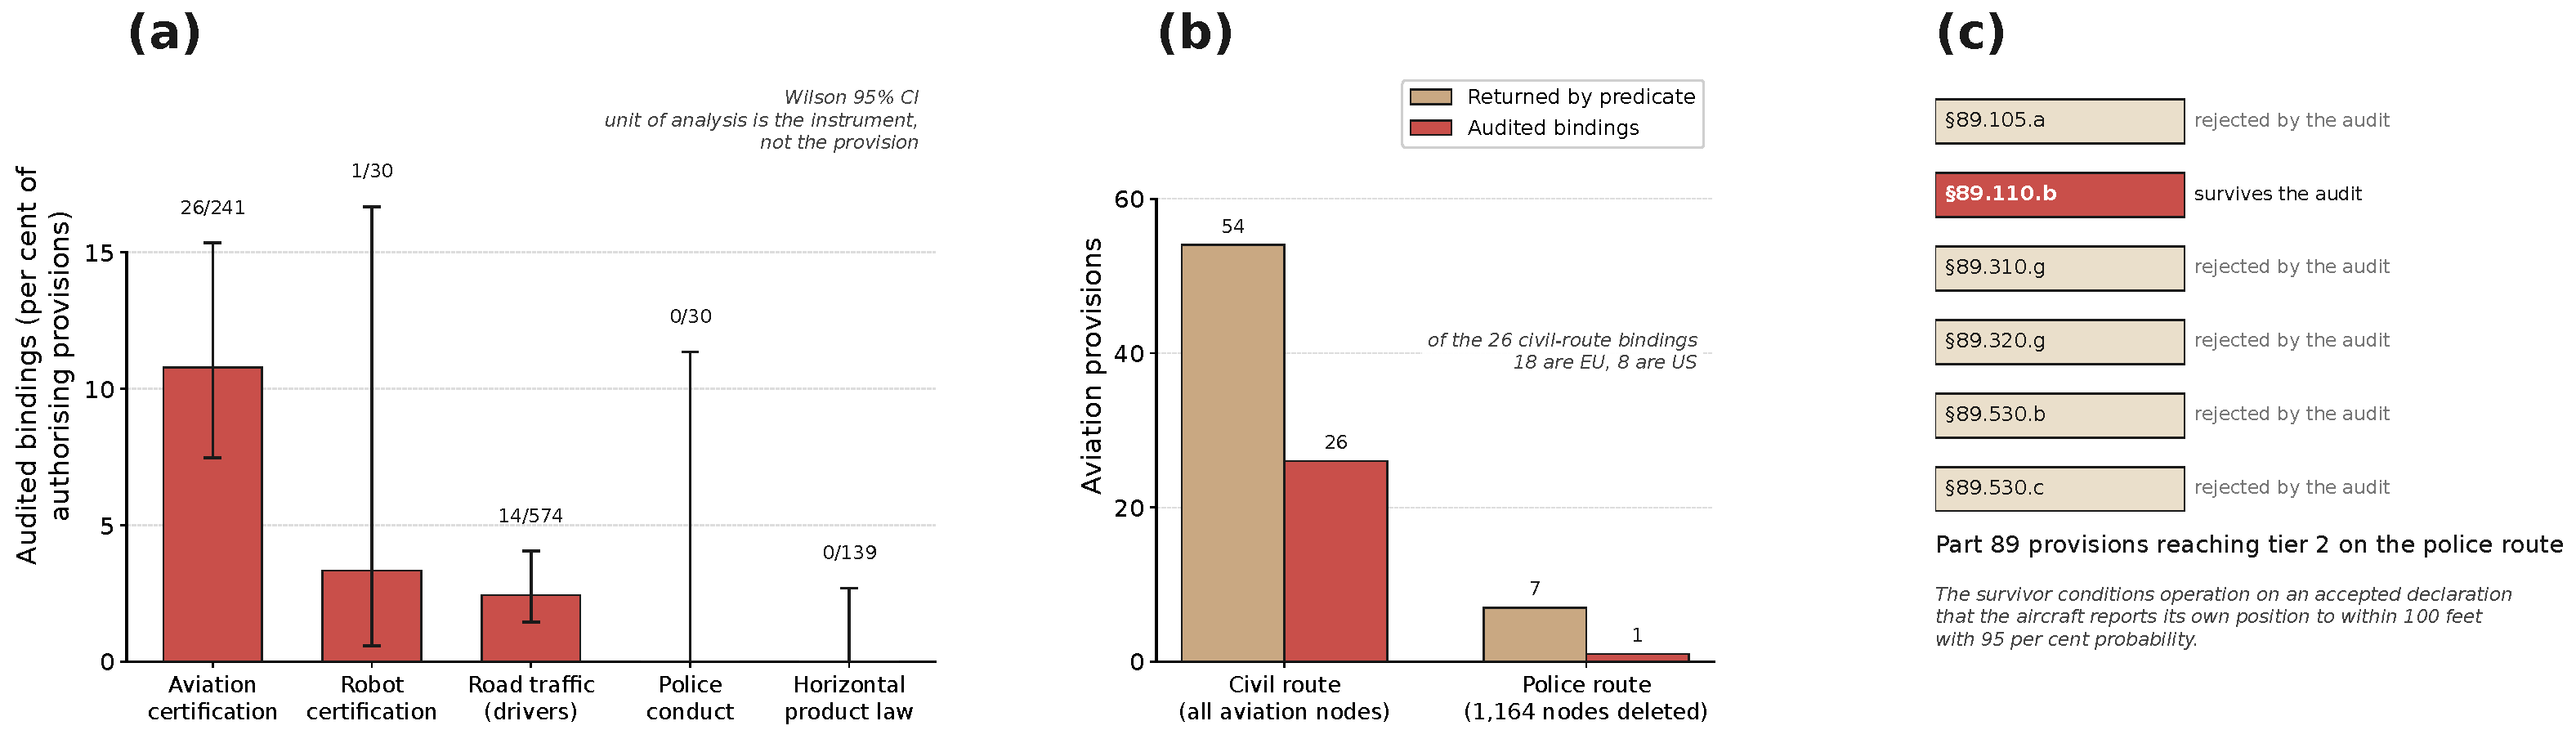
\includegraphics[width=\textwidth]{FigR}
\caption{Where audited bindings are, and what a police exemption removes. (a) Audited bindings as a share of authorising provisions, by subject matter, with Wilson 95\% intervals and the count over the total above each bar. The partition is the post-hoc one of Table 8. The rates are descriptive: the unit of analysis is the instrument, not the provision, and at instrument level the domains do not separate, so the panel carries the clustering statistics rather than a test (Section 3.3). The two cells of 30 provisions are shown for composition. (b) The same airframe adjudicated on the civil route and with the police and public-aircraft carve-outs applied as deletions of 1,164 of the 5,758 nodes in the provision graph, everything else held constant; the returned counts are 54 and 7, the audited counts 26 and 1. Of the 26 civil-route bindings, 18 are EU and 8 are US; the EU deletion removes all 1,047 nodes of the three EU instruments, while the US deletion is selective and leaves 306 aviation nodes holding 34 authorising provisions in force, among which one binds. (c) What the exemption leaves. 6 provisions of Part 89 reach tier 2 on the police route and one, \S{}89.110(b), survives the audit: it conditions operating a standard remote identification unmanned aircraft on an accepted declaration that the aircraft reports its own position to within 100 feet with 95 per cent probability. Part 89 was made in 2021, after the public-aircraft doctrine was settled, and is not among the instruments AC 00-1.1B exempts.}
\label{fig:f3}
\end{figure*}

operator is only if, and the object of the condition is a named evaluation named in the same paragraph. It satisfies all three audit conditions, and it survives the disjunction test of Section 2.7: requirement (b)(2) independently demands that the aircraft's remote identification equipment be functional and comply with this part, and \S{}89.125 bars ADS-B Out from being used to comply with the remote identification requirements of this part, so the one branch of (b)(1) that would otherwise bypass \S{}89.310 is closed by a requirement conjunctive with it.

The content of that declaration is fixed four provisions away, and the chain is worth setting out because the content of the evaluation is the whole of the finding. Section 89.530(a) requires the producer of a standard remote identification unmanned aircraft under \S{}89.515 to submit a declaration of compliance for FAA acceptance. Section 89.515(a) requires such an aircraft to be designed and produced to meet the minimum performance requirements established in \S{}89.310. And \S{}89.310(h)(1) requires that the reported geometric position of the unmanned aircraft and the control station be accurate to within 100 feet of the true position, with 95 percent probability. The alternative branch of \S{}89.110(b)(1), a part 21 design or production approval plus the requirements of Subpart F, runs through \S{}89.510(b)(1) to the same section, but \S{}89.510(b) is itself disjunctive and its branch (2) is satisfied by ADS-B Out equipment meeting \S{}91.225, which reaches no evaluation. That branch is closed not by requirement (1) but by requirement (2) of \S{}89.110(b), which demands independently that the aircraft's remote identification equipment be functional and comply with this part, read with \S{}89.125, which provides that ADS-B Out equipment cannot be used to comply with the remote identification requirements of this part. We set the reasoning out because the audit split on it, one pass labelling the provision a binding and one not, and because \S{}91.225 lies outside the corpus so we cannot say from the measured text whether it names an evaluation of its own.

So where a police unmanned aircraft is operated as a standard remote identification unmanned aircraft, the permission is conditioned on how accurately it reports where it is. It is not the only route. Section 89.105 makes \S{}89.110 one of three ways to comply, the others being a broadcast module under \S{}89.115(a), which reaches the same kind of declaration through \S{}89.320, and operation inside an FAA-recognized identification area under \S{}89.115(b), which requires no remote identification equipment and no evaluation at all; \S{}89.105 also opens with an exception for operations the Administrator otherwise authorises. An earlier version of this paper called \S{}89.110(b) the authorisation a police unmanned aircraft must earn, which overstates it. What the measurement supports is that \S{}89.110(b) is the only binding in force on the police route, not that every police operation must pass through it.

Two things must be said about that chain. The first is that it is a reading of the text and not a measured path: the provision graph holds no edge from \S{}89.110(b) to \S{}89.310(h), because \S{}89.110(b) names the declaration of compliance as a term rather than as a numbered crossreference, and the predicate scored the provision tier 2 on the evaluation term in its own paragraph. We verified each link of the chain against the corpus text and release the check; we do not claim the graph found it. The second is what the threshold is about. One hundred feet at 95 per cent probability is a requirement on the broadcast position of the airframe. It says nothing about the accuracy of a chemical identification, a thermal reading, a face match or any other sensing on which a police decision might rest. The corpus contains no provision in force on the police route that conditions an authorisation on an evaluation of that kind, and the sweep of Section 3.5 is the independent check on that statement.

How the total is composed. Without this, the 25 reads as stronger than it is. The EU and US carve-outs are not the same kind of operation, and the 25 is a sum across two bodies of law that

no single aircraft is subject to at once. Split by jurisdiction, the EU side contributes 18 audited bindings on the civil route and 0 on the police route, and the deletion there removes all 1,047 nodes of Regulations 2018/1139, 2019/947 and 2019/945, leaving nothing of the EU aviation corpus behind. That is close to analytic: Article 2(3)(a) excludes police activities from the basic act, so the acts resting on it go with it, and a binding cannot survive in a text that is no longer in scope. The US side contributes 8 audited bindings on the civil route and 1 on the police route, and there the deletion is selective. It removes Subparts C and D of Part 107 and leaves 306 aviation nodes standing: the rest of Part 107, the whole of Part 89 and the advisory circular itself. The one surviving binding is in those 306 nodes. The informative measurement is there, not in the EU column, and we report the two separately for that reason.

The retained population. Three facts about the remainder are needed before any null is read. The first is its size in the paper's own unit. The 306 retained aviation nodes contain 34 authorising provisions, 17 in Part 89, 12 in the retained subparts of Part 107 and 5 in the advisory circular; the police route as a whole retains 807 authorising provisions of the 1,014, because the carve-out touches only the aviation instruments. Node counts and provision counts are not interchangeable and we give both.

Two of those three components are retained on grounds that do not hold, and the direction of the error matters. Part 107 applies, by \S{}107.1(a), to civil small unmanned aircraft systems, and 49 U.S.C. \S{}40102(a)(16) defines a civil aircraft as an aircraft other than a public aircraft; AC 00-1.1B says in terms that regulations whose applicability uses the phrase civil aircraft do not apply to public aircraft operations. On that reading the whole of Part 107 leaves the police route, not merely Subparts C and D, and the 12 retained Part 107 provisions go with it. The five advisory-circular provisions should not be in the authorising population at all: Section 2.3 declares guidance excluded and retains AC 00-1.1B only as the documentary basis for the carveout rule, and their presence is a failure to execute that exclusion, which we report rather than repair after the fact. The defensible retained population is therefore Part 89 alone, 17 authorising provisions, and the surviving binding is in it.

Every one of these choices was made in the direction that retains, which makes the police route look better covered than it is. Correcting them shrinks the retained population and leaves the result unchanged: the single surviving binding is in Part 89, which no one disputes remains applicable. Removing the five advisory-circular provisions also moves the nominal aviation rate from 10.8 per cent to 11.0 per cent, 26 of 236, which no conclusion turns on.

The second is the tier distribution of Part 89, which is where a counterexample would have to live, since Part 89 is the one aviation instrument the carve-out leaves entirely intact. Of its 17 authorising provisions, 6 reach tier 2: \S{}89.110(b), which is the binding, and five the audit rejects. Those five are \S{}89.105(a), which fails the disjunction test because its condition is satisfied by operating inside an FAA-recognized identification area under \S{}89.115(b) with no remote identification equipment and therefore no evaluation; \S{}\S{} 89.310(g) and 89.320(g), where the only evaluation term is a date reference, naming the date a declaration of compliance is submitted; and \S{}\S{} 89.530(b) and (c), which impose a declaration duty on a producer and list the information the declaration must carry. Two reach tier 1 and 9 reach tier 0. The two at tier 1 are \S{}89.115(a) and \S{}89.505(a). Two earlier versions of this distribution were wrong and both are reported in Section 2.10. The first listed \S{}89.530(i) at tier 1; no such provision exists in 14 CFR, and the entry was an artefact of the extraction defect that promoted \S{}89.530(c)(7)(i) to a top-level paragraph. The second, published through the eighth review round, gave the population as 20 and named four tier-1 provisions, two of which, \S{}\S{} 89.510 and 89.515, are section captions with paragraph children and were in the population only because the paragraph-node rule was not being enforced on United States identifiers. They reach a named evaluation through the same declaration-of-compliance chain as the binding and fail the predicate on the operator rather than on the evaluation: the obligation in each is on the producer, and the operating rule refers to equipment already produced under an accepted declaration without itself conditioning a grant of permission on an outcome. Section 89.110(b) differs from them in exactly one respect, which is that it addresses the operator and conditions the operation. We report the whole distribution rather than only the returns, because a reader checking the defeater of Section 2.10 should not have to take it on trust that nothing else in Part 89 reaches tier 2.

The third is recall on this population, and it is the weakest part of the paper. The lexicon projection of Section 2.6 gives a false-negative rate within a tier-1 population, and recall follows from it only if the audited bindings in the numerator and the tier-1 provisions in the denominator are drawn from the same population. Two earlier versions of this paper failed that condition in opposite directions and both are withdrawn. The first reported a recall of 88.6 per cent, which is one minus the false-negative rate and is not recall at all. The second divided one audited binding, which is the aviation survivor, by a projection taken over the whole police route, and reported the result as a recall of 1 in 43; the numerator was aviation and the denominator was not.

Matched populations give the following. On the police route as a whole there are 16 audited bindings and 367 tier-1 provisions, so the projection is 46 missed bindings with an interval of 17 to 108 and recall is 0.26 [0.13, 0.48]. On the aviation part of the police route, which is where the surviving binding and the negative claim both sit, there is 1 audited binding and 10 tier-1 provisions, the projection is 1.3 [0.5, 2.9] and recall is 0.44 [0.25, 0.68] on a population too small to carry weight. Corpus-wide, 41 audited bindings against 491 tier-1 provisions give a projection of 62 [23, 145] and recall 0.40 [0.22, 0.64]. The corrected figures are better for this paper than the withdrawn 1 in 43 by roughly an order of magnitude, which is the direction that obliges us to state plainly that the error was ours and that it understated our own instrument. The negative claim this paper makes is therefore bounded accordingly: what the measurement establishes is that the only binding the predicate can see on the police route conditions the aircraft's report of its own position, and that the predicate's recall on that population is low enough that the claim must be read as a statement about what a frozen, published, audited rule finds rather than as a census of the law.

\subsection{The legal form that would bind sensing performance exists and enumerates its scope}\label{sec:3.5}

Directive 2014/32/EU is the European legal-metrology regime, and it does, on its face, exactly what this paper has been asking whether any instrument does. We set out that reading before qualifying it, because the qualification matters: the provision in question is one of the 57 the audit rejected, and what follows is therefore a legal reading of the Directive, not a measurement of it. Article 7(2) requires Member States to take all appropriate measures to ensure that measuring instruments are made available on the market and/or put into use only if they satisfy the requirements of the Directive, and Annex I states that the error of measurement shall not exceed the maximum permissible error laid down in the instrument-specific requirements. A permission is conditioned determinately on a stated metrological performance.

Article 2(1) then enumerates what the Directive applies to: water meters (MI-001), gas meters and volume conversion devices (MI-002), active electrical energy meters (MI-003), thermal energy meters (MI-004), measuring systems for continuous and dynamic measurement of liquids other than water (MI-005), automatic weighing instruments (MI-006), taximeters (MI-007),

material measures (MI-008), dimensional measuring instruments (MI-009) and exhaust gas analysers (MI-010).

No category is a law-enforcement measuring instrument. No category is a chemical, biological, radiological or nuclear detector, an airborne sensing payload, or any instrument whose reading supports a police determination. The form that would close the gap is neither missing nor immature. It has existed in its present shape since 2014 and in its predecessor since 2004, and its scope was drawn by enumeration.

Two qualifications are owed on this subsection, and both run against us. The first is the one stated above: Article 7(2) is a provision the audit rejected. The predicate reached its evaluation term in the definitions of Article 4 rather than in Annex I, and the chain drawn in Fig. 4a is the chain a lawyer reads, not the path the predicate recorded; with the unnumbered structural edges removed the provision falls to tier 0. We had described this instrument as a positive control demonstrating that the predicate finds the structure when it is present, and that description does not hold. A third point runs the same way and is owed to the reading above. Article 7(2) obliges Member States to take all appropriate measures to ensure that instruments are made available or put into use only if they satisfy the Directive, and that is the same form of qualification the next subsection uses to reject AI Act Article 15. The hedge list of Section 2.6 carries as appropriate and where appropriate but not this phrase, so the predicate did not treat it as a hedge. Adding the phrase to that list is a one-line change whose measured effect is to move Article 7(2) to tier 1 and the returned count from 91 to 90, leaving the audited bindings unchanged. We report the omission rather than repair it after the fact, and note that the repair would remove the only provision this subsection discusses from the returned set altogether. The second is that Article 3, headed Optionality, provides in paragraph 1 that Member States may prescribe the use of measuring instruments for measuring tasks where they consider it justified for reasons including public safety and public order, so Article 2(1) enumerates the categories for which Union-level requirements exist rather than the whole set of instruments subject to legal metrology. The enumeration is a boundary of competence as much as a boundary of legislative attention, and the Korean Measurement Act we were unable to retrieve belongs to precisely the national layer this qualification points at.

\subsection{The closest thing to a counterexample, and why it is not one}\label{sec:3.6}

A negative result is only as good as the search that failed to refute it, and the lexicon projection of Section 2.6 bounds how many bindings of any kind the predicate misses without saying whether a missed one would concern sensing performance. We therefore ran a second search that does not use the predicate at all. Seventeen concepts of measurement and sensing performance were matched against the text of all 5,758 provision nodes: maximum permissible error, measurement error, accuracy, precision, detection limit, false positive and false negative rate, sensitivity, specificity, calibration, metrology, tolerance, uncertainty, repeatability, reproducibility, resolution, a stated performance standard, and the construction within n feet, metres or seconds. Each concept is expressed in all three languages of the corpus, and the search script asserts that before it runs, so a concept cannot be present in English and absent in Korean or Japanese. The seventeen concepts expand to 78 patterns, 23 English, 30 Korean and 25 Japanese, matched on word stems rather than exact forms.

Two changes widened this sweep and both are reported. An earlier version matched whole words and therefore missed accurate where it had looked for accuracy. A later version, the one reported through the eighth review round, had stemmed the English entries but left the Korean and Japanese entries as bare nouns, so no Korean or Japanese node matched at all and the

\begin{figure*}[!t]
\centering
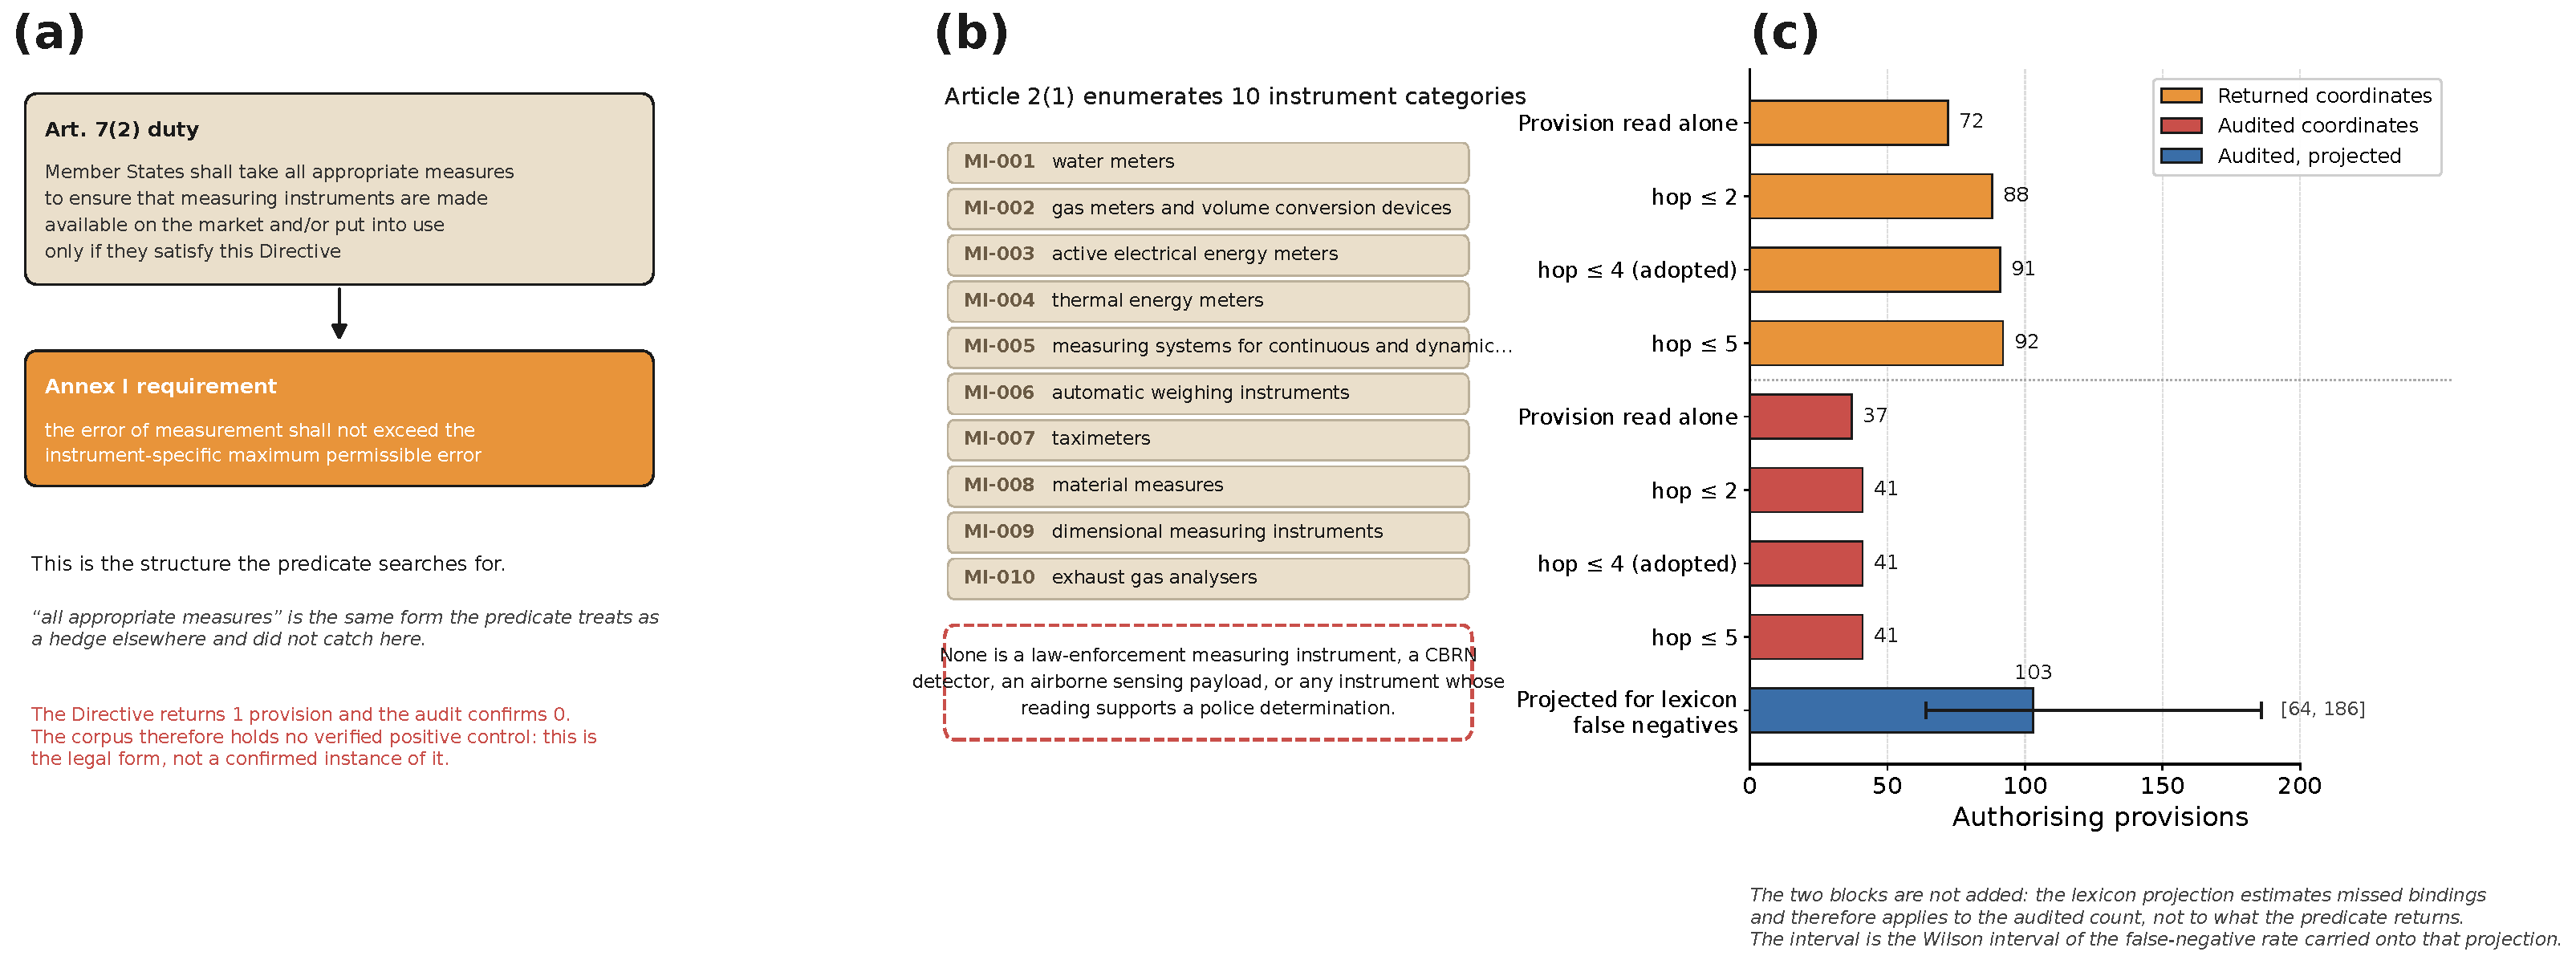
\includegraphics[width=\textwidth]{FigS}
\caption{The legal form that would bind sensing performance, its enumerated scope, and the robustness of the count. (a) The binding chain in Directive 2014/32/EU: Member States are to take all appropriate measures to ensure that instruments are made available on the market and/or put into use only if they satisfy the Directive, whose Annex I requires that the error of measurement not exceed the instrument-specific maximum permissible error. This is the structure the predicate searches for. The qualification on the Member State duty is shown because it is the same form the predicate treats as a hedge elsewhere and did not catch here, as Section 3.5 records. The Directive's single returned provision is rejected by the audit of Section 2.7, so the corpus contains no verified positive control and the chain is shown as the legal form rather than as a confirmed instance of it. (b) Article 2(1) enumerates the ten instrument categories the Directive applies to. None is a law-enforcement measuring instrument, a chemical, biological, radiological or nuclear detector, an airborne sensing payload, or any instrument whose reading supports a police determination. The gap is not an immature legal form; it is a boundary that was drawn. (c) The count under each variant of the rules that produced it. The upper block is in returned coordinates and the lower block in audited coordinates; the two are not added, because the lexicon projection of Section 2.6 estimates missed bindings and therefore applies to the audited count of 34, not to the 91 the predicate returns. The interval on the last row is the Wilson 95\% interval of the false-negative rate carried onto that projection.}
\label{fig:f4}
\end{figure*}

claim that the sweep covered three languages described the pattern list rather than the evidence. Symmetrising the three languages is the repair, and it is the same repair the determinacy lexicon received at the v14 refreeze; that it was still needed here is reported in Section 4.6.

These patterns occur in 51 of the 5,758 nodes, of which 21 are in the metrology Directive and six are Korean or Japanese. Among the 1,014 authorising provisions they occur in 12, and none of the 12 is a provision the predicate returns: seven are tier 1 and five tier 0. The symmetrisation added six nodes and no authorising provision, so it widened the search without changing what the search found. Those six deserve saying plainly, because a reader could take them for Korean and Japanese evidence that the sweep now has. They are not. All six match the accuracy concept in a non-measurement sense: closing a door accurately, operating the steering and braking controls accurately, operating an outdoor delivery robot's controls accurately, keeping records accurately in two driving-school provisions, and recording an operating state accurately. None is a performance condition and none is an authorising provision. After symmetrisation the Korean and Japanese contribution to this sweep is still empty, and the sweep's evidence remains English. Read one by one, none conditions an authorisation on a measured performance. Three concern the supplementary metrology marking, where it is affixed and that a distributor must check it is present (Articles 11(2), 22(3) and 22(5) of Directive 2014/32/EU). Three are in Implementing Regulation (EU) 2019/947, where accurate and precise qualify the information an operator must supply or the position a geo-awareness function must use, not a permission. One is the phrase calibrated air speed in Regulation (EU) 2018/1139 Article 2(8), a unit of measurement inside an aircraft category threshold, and one is the definition of measurement uncertainties in Regulation (EU) 2019/945 Article 3(35). One requires the holder of a Confirmation of Identification to keep its information accurate (14 CFR \S{}89.130(d)), and one requires that AI-generated content be marked in a machine-readable and detectable form (AI Act Article 50(2)). The remaining two are Article 4(1) of the Law Enforcement Directive, which requires personal data to be accurate, and Article 13(3) of the AI Act, which is the only substantive candidate among authorising provisions and is treated next.

An earlier version of this paper described two of these as the definition of a conformity assessment body in Regulation (EU) 2019/945 Article 3(1) and the definition of legal metrological control in Directive 2014/32/EU Article 4(1). Both citations were wrong, and wrong for the same reason: the extractor held each definitions article whole, so the node identifier \texttt{art\_3.1} meant the article rather than its first definition. Article 3(1) of Regulation (EU) 2019/945 defines unmanned aircraft; conformity assessment body is Article 3(11). Article 4(1) of Directive 2014/32/EU defines measuring instrument; legal metrological control is Article 4(3). The repair reported in Section 2.10 splits those articles into their numbered definitions, which is why neither now appears among the authorising provisions at all.

Three of the 51 nodes fall in Part 89, and they are the reason this subsection no longer reads as a flat negative. One is \S{}89.130(d), listed above. The other two are \S{}\S{} 89.310(h) and 89.320(h), the message-element performance requirements, which state the only numeric performance thresholds the sweep finds anywhere in force on the police route: the reported geometric position accurate to within 100 feet with 95 per cent probability, the reported geometric altitude to within 15 or 150 feet on the same probability. Neither is an authorising provision, and neither is reached from \S{}89.110(b) by any edge in the graph, but \S{}89.110(b) reaches both by the textual chain of Section 3.4. The sweep therefore confirms, from an instrument independent of the predicate, both halves of this paper's finding: a stated performance threshold does condition an operating permission on the police route, and the property it governs is the aircraft's report of its own position rather than anything the aircraft senses about the world. No pattern in the sweep

matches a provision that conditions a permission on the accuracy of a chemical, biological, radiological, thermal, acoustic or visual determination, in any of the sixteen instruments, on either route.

Article 13(3) requires the provider to state, in the information accompanying a high-risk system, the level of accuracy against which the system has been tested, and the accuracy it points to is set by Article 15. Article 15 is therefore the strongest candidate anywhere in the corpus. It does not appear among the twelve because it is not an authorising provision, which is the first thing to say about it; the reason it fails on the merits is worth stating as well, because it is the reason the paper's whole construct is built the way it is. Article 15(1) provides that high-risk AI systems shall be designed and developed in such a way that they achieve an appropriate level of accuracy. The operator is mandatory. The standard is not: appropriate is the hedge the predicate is defined to catch, and Article 15(2) confirms the reading by charging the Commission with encouraging the development of the benchmarks and measurement methodologies by which such a level would be measured, which is a statement that they do not yet exist. Article 15(3) requires only that the levels and metrics be declared in the instructions for use, and Article 13(3)(b)(ii) carries that declaration into the information the provider supplies. None of Article 15(1) to (3) is an authorising provision at all: they impose design and disclosure duties on a provider and confer no permission, so they do not enter the population this paper measures, and Article 15(4) and (5), which do, reach no evaluation. The AI Act thus contains the vocabulary of measured performance, attached to a duty on a manufacturer and hedged, and does not attach it to the authorisation under which a police agency deploys the system.

Article 15 is not the only place a counterexample could be, and the conformity-assessment machinery of Article 43 has to be examined before the claim can be made for the instrument as a whole, because that is where a permission would be attached to an assessment if it were attached anywhere. Paragraphs (1) to (3), (5) and (6) are not authorising provisions on the predicate's reading: they direct a provider to a procedure rather than conferring a permission, and paragraph (1) hedges with may in any case. Paragraph (4) is an authorising provision and reaches tier 1, mandating a fresh assessment after a substantial modification without conditioning anything on a determinate operator. Paragraph (3) is the one that merits adjudication rather than a tier. It provides that where a listed act lets a manufacturer opt out of third-party assessment, that manufacturer may use that option only if it has applied the harmonised standards and common specifications covering the requirements of Chapter III Section 2. The predicate does not return it, because may use that option is not in the authorising lexicon; adding that phrase is a one-line change whose measured effect is to return Article 43(3) at tier 2 and move the returned count from 91 to 92. We report the omission rather than repair it, and the reason is that the provision fails the audit on its merits in a way that is worth more than the count. Conditions (i) and (ii) hold: a permission is conferred and a determinate operator conditions it. Condition (iii) fails, and it fails twice over. What only if conditions is the application of harmonised standards, which is a declaration about process rather than a named evaluation procedure; and the assessment named in the same sentence is the one the manufacturer is permitted to opt out of. The strongest determinate conditioning of a permission in the AI Act therefore conditions the avoidance of an assessment, not the passing of one.

What lies behind Article 43 reinforces this, and it is a legal reading rather than a measurement, because the annex truncation described below removes it from the corpus. Article 43(2) routes the high-risk systems of points 2 to 8 of Annex III to the conformity assessment procedure based on internal control in Annex VI, and says in terms that this procedure does not provide for the involvement of a notified body. Point 6 of Annex III is law enforcement. Annex VI, 1,211

characters in the published text, defines that procedure as three acts of the provider upon its own system: it verifies its quality management system against Article 17, examines its own technical documentation against the essential requirements, and verifies that its design and post-market monitoring are consistent with that documentation. No performance threshold appears in it. The route by which a law-enforcement AI system reaches the market under the AI Act is therefore provider self-verification against a standard that Article 15 leaves hedged, with no third party and no stated metric. This is the same structure the paper reports for the police route in aviation and on the ground, reached independently and in the instrument that was the likeliest place to find the opposite.

This is the bound we can offer on the negative claim that the lexicon projection cannot, and it is narrower than it first appears, in two ways we should state. A binding may reach a performance threshold without naming one, by requiring a conformity assessment that delegates the threshold to a referenced standard, and that is the dominant form among the 23 aviation bindings we do count; the sweep would not see such a provision unless the delegating text itself used a performance term, and \S{}89.110(b) is an instance of exactly that: the sweep matches the threshold node but not the authorising provision that reaches it. Annexes are truncated at 6,000 characters, so the pages where thresholds are actually tabulated, including the instrument-specific tables of the metrology Directive, are largely outside the text the sweep reads. What the sweep therefore establishes is the absence of a provision that states a sensing performance condition anywhere in the corpus, authorising or not, not the absence of one that reaches such a condition by delegation. Within that scope it is a real bound, and a narrower opening than the 23 to 145 missed bindings of any kind that Section 2.6 projects.

\subsection{The result survives the choices that could have produced it}\label{sec:3.7}

Path bound. Returned counts saturate at four hops; the fifth adds one across the corpus, and removing the unnumbered structural and chapter edges entirely changes the count from 91 to 89 (Table 2). Audited counts saturate earlier, at two hops (Table 7). The bound was frozen before the audit and is not revised in the light of it, but the audited column shows that relaxing it past two hops buys no binding and costs precision at every step.

Scope restriction. A constraint derived from one mission may only match instruments in that mission's domains. This was the most outcome-determining discretionary choice in the earlier design, and it is worth saying what became of it: the restriction operates only where a constraint is matched to instruments, and no quantity reported in this paper passes through that step. The predicate runs over all 1,014 authorising provisions in all sixteen instruments regardless of which mission motivated the study, so the domain rates, the path variants, the carve-out comparison and the audit are unaffected by it. Reporting its effect would require the constraint-level counts that Section 3.8 withdraws, so we do not report one.

Hedge rule. A path is capped when any node on it carries a hedge. Because nodes are paragraphs, a paragraph in which a determinate condition and a hedge govern different clauses is capped even though the condition stands, and this can only remove bindings, so it biases towards our own conclusion. Removing the cap entirely, the most generous variant the rule admits, raises the returned count corpus-wide from 91 to 116 (Fig. 4c). An earlier version of this paper added that the 25 new returns contribute no audited binding. That statement is withdrawn as a sensitivity result, because it is true by construction rather than by measurement: the audit population is the 91 returns of the adopted rule, so none of the 25 carries a label and none could have been counted as a binding. What the row establishes is the size of the returned set under the most generous

reading of the hedge rule, and it is silent on how many of those returns would survive an audit. The same applies to the hop $\le$ 5 row, whose single additional return is likewise unlabelled.

Lexicon. The validated false-negative rate in the tier-1 population is 12.6\% [4.7, 29.5], and none of the observed false negatives concerns sensing or measurement performance (Section 2.6). Two statements an earlier version made about that rate are withdrawn. It is not a ceiling on the instrument's miss rate but a floor, because the validation samples only tier 1. Tier 0 was sampled separately and later (Section 2.10), and what it returned was not a missed binding of the kind the validation looks for but a missing class of lexicon terms; repairing that moved four Japanese provisions from tier 0 into the audited set, which is itself a measurement of how much the tier-1 rate understates the whole. And the absence of a language penalty is not shown: English returns 2 of 12 against 2 of 22 for Korean and Japanese together, Fisher exact p = 0.60, and a simulation puts the power of that comparison at 0.07 against a non-English rate of 30 per cent. That is an absence of power, which Section 3.3 refuses to read as equivalence elsewhere, and we refuse it here. The rate is a floor on the instrument and it is a low one: carried onto the audited counts it implies a recall near a third corpus-wide and far lower on the police route (Section 3.4). Separately, the lexicon contained a defect that no sensitivity in this list would have caught, because it suppressed a construction rather than mis-scoring one; it was found by testing the paper's own defeater and is reported with its effect in Section 2.10.

Corpus composition. The two instruments added after freezing are the two most likely to refute the paper. Both are reported above and neither refutes it. We no longer claim, as we did, that the metrology directive supplies a positive control demonstrating that the predicate finds the structure when it is present: its one returned provision is rejected by the audit, and the corpus therefore contains no verified positive control. This is a weakness of the instrument and we state it as one.

Audit. Precision is 0.451 [0.352, 0.553] over the returned set and differs by domain (Section 2.7). Every returned provision was labelled in two passes by one investigator using a language model as the instrument, so what the agreement figures measure is repeatability of the procedure and not agreement between readers. Agreement over all 74 labelled records is 51, $\kappa$ = 0.448 against a marginal ceiling of $\kappa$max = 0.520, with Gwet's AC1 at 0.577; outside the single ambiguous sentence pattern agreement is 51 of 56, which is the residue after the disputed cell is deleted and estimates nothing. Those 74 are the records both passes saw. One of them left the returned set under the lexicon symmetrisation of Section 2.10, and 18 records entered it after the passes were complete, so the agreement figures describe 74 records of which 73 are in the current returned set of 91 and none of the 18 later entrants is included. The audit was performed after the ruleset was frozen and no rule was changed in response to it.

Denominator. The authorising population is itself audited at 0.494 [0.386, 0.602] and the contamination is uneven, heaviest among the cross-cutting instruments (Section 2.8). Every rate is therefore reported in both coordinates. Correcting the denominator moves every rate upward and widens the aviation-to-ground contrast, so the nominal pair is the conservative one and no conclusion turns on the choice.

Determinism. The adjudication re-runs bit-identically from the frozen ruleset across hash seeds, and the corpus files verify against their recorded hashes.

\subsection{Why constraint-level counts are not reported}\label{sec:3.8}

The earlier design of this study reported outcomes for each of the 63 derived constraints. Doing so requires translating each constraint into search terms for four legal systems, and that

step is performed by a person rather than by the predicate. We tested whether it is reproducible. Twelve constraints were drawn at random, and the constraint sentences, the corpus and the termwriting rules were given, with nothing else, to a second term-writing pass made without access to our term lists, our results or this manuscript. The pass was executed by the same investigator using a large language model, so it measures the stability of the step under re-execution from the written rules rather than agreement between two people; it is the weaker of the two readings, and the result is poor under either. Applying the re-written terms through the same adjudicator reproduced our outcome class for 5 of 12 constraints. The outcome class takes four values, which are the ones the adjudicator can return: no concept reached, no determinate binding, not an authorising provision, and determinate binding. Our register produced 8, 3, 1 and 0 of them; the re-written register produced 3, 5, 2 and 2. On that scale Cohen's $\kappa$ is 0.184, with po = 0.417 and pe = 0.285. The full cross-tabulation is in Table 10, and we give it because a $\kappa$ on 12 cases and four classes is not interpretable without one: the number is reported as evidence that the step is unreliable, not as an estimate of how unreliable.

\begin{table}[!htb]
\centering
\caption{Outcome classes for the twelve held-out constraints, our register against the blind re-written register. Agreement is the diagonal, 5 of 12. Blind re-written register}
\label{tab:t10}
\small
\begin{tabular}{@{}lrrrr@{}}
\toprule
Our register & No concept & No binding & Not authorising & Binding \\
\midrule
No concept reached & 3 & 2 & 2 & 1 \\
No determinate binding & 0 & 2 & 0 & 1 \\
Not an authorising provision & 0 & 1 & 0 & 0 \\
Determinate binding & 0 & 0 & 0 & 0 \\
\bottomrule
\end{tabular}
\end{table}

The disagreements are instructive and symmetric. The re-written terms returned a determinate binding in two places where ours did not. The first is the headline constraint of the earlier design, which we had scored as reaching no determinate path; inspection shows the match is an artificial-intelligence classification provision reached through generic terms. The second is a constraint for which our terms returned no match at all while the re-written terms returned sixteen; inspection shows those sixteen to be driving-licence surrender provisions in the Japanese and Korean road-traffic law, matched through a grammatical particle. Neither register dominates: both produce false positives, in different places, and the re-written register produces them in the direction that would refute this paper.

We therefore report no constraint-level counts in this paper. The constraint registers are published because they document what the missions demand and are reusable, but the measurements above are confined to quantities that no analyst-written search term enters: the domain rates in Tables 9 and 8, the path contribution, the carve-out comparison, and the scope of the metrology Directive. This is a reduction in what we claim relative to the earlier design, and it is the reduction the reliability measurement requires.

\section{Discussion}\label{sec:4}

\subsection{Two regimes, one object each, and a gap between them}\label{sec:4.1}

The corpus is not silent about police robots. It contains 1,014 authorising provisions, of which the predicate returns 91 and the audit confirms 41, and the instruments that produce them

are recent, specific and enforceable. What the measurement shows is that those 41 bindings attach to three objects, and that the object a deployment decision turns on is none of them.

The first object is the machine as an article of commerce. Airworthiness, type certification, conformity assessment and market access account for 6 of the 41 audited bindings, assessed before sale, by a body external to the buyer, against thresholds fixed in advance. That is a minority, and an earlier version of this paper had it as the majority; the classification of Section 3.3 measures 35 of the 41 as conditioning an operating permission instead. The correction matters for how the gap should be described. Law does not confine itself to the point of sale and leave use alone. It conditions use heavily, on pilot licences, operator certificates, aerodrome certificates, operational authorisations and the airframe's own compliance, and the property it conditions use on is never a sensing performance. The second object is the purpose of the police act. The Law Enforcement Directive, the AI Act's law-enforcement provisions and the municipal and state equipment-governance instruments are precise about why a capability may be used, who must approve it and what follows from a breach. Between them lies the proposition that the reading on which an officer acts has been shown to be adequate for the conditions of use. No audited binding occupies that space. The three instruments that regulate police conduct return none in their 30 authorising provisions, and the two horizontal product instruments return three in 139, all rejected by the audit.

The third object is the one this paper discovered by failing to refute itself, and it is the smallest of the three: a single provision, 14 CFR \S{}89.110(b), conditions permission to operate on an accepted declaration that the aircraft reports its own geometric position to within 100 feet with 95 per cent probability (Section 3.4). Most of the audited bindings condition operating rather than selling, so that is not what distinguishes it; what does is that it is the only one of the 23 aviation bindings that survives the police carve-out. Its object is the machine's account of its own location. This is a performance property, it is stated numerically, it is tied to a permission determinately, and it concerns the aircraft as a thing to be found in the sky rather than as an instrument that produces a reading an officer will act on. The gap this paper describes is therefore not a gap between regulation and silence. It is a gap between the properties of a police robot that law has learned to condition permissions on and the property a police decision actually rests on, and those two sets intersect in exactly one provision concerning neither the robot's sensing nor the officer's use of it. The police-conduct zero rests on 30 provisions and is reported in Section 3.3 as a reading of their text rather than a statistical contrast.

The regulatory-design literature explains why the division falls where it does. Kaplow's distinction between rules and standards turns on when the content of the law is fixed \citep{Kaplow1992Rules}, and Diver's account of optimal precision adds that precision is costly and is therefore bought where the rulemaker can bear the cost of being specific \citep{Diver1983Precision}. Specifying in advance what sensing performance suffices for a police determination requires the rulemaker to know the mission, the analyte, the environment and the consequence. Specifying that a permission depends on a purpose and a prior authorisation requires none of that. Coglianese and Lazer's account of management-based regulation describes what is written instead: the regulated party must plan, assess and document, and the regulator supervises the process \citep{CoglianeseLazer2003}. Such supervision is a reasonable response to heterogeneous technology, and it is precisely the form our predicate records as indeterminate.

\subsection{The asymmetry runs between certification and conduct, not between aviation and the ground}\label{sec:4.2}

The pooled comparison between aviation at 10.8\% and the ground corpus at 2.5\% invites the obvious explanation, that aviation certification is a century old and ground robotics is not. We

cannot offer that explanation, because we cannot defend the comparison it would explain. The ground category pools two bodies of law that have no reason to behave alike, and 95\% of its denominator is human driver licensing (Section 3.3). Splitting it does not rescue a different comparison either: the Korean robot instruments supply 30 authorising provisions and 1 audited binding, and a cell that size cannot distinguish the aviation rate from the road-traffic rate in either direction.

The densest contrast is aviation certification against road-traffic law, 26 of 241 against 14 of 574, and it is large in the descriptive sense established in Section 3.3 rather than in a tested one. That is a contrast between a regime built to condition a permission on a demonstrated property of a machine and a regime built to condition a permission on a demonstrated property of a person. The ground bindings are driving examinations and aptitude tests; the aviation bindings are airworthiness and conformity assessment. Whether robot certification behaves like the first or the second is a question this corpus is too small to answer, and we leave it open rather than answering it from two events.

Two explanations of the aviation result itself have to be set aside. The first is a language artefact: an earlier version of this paper reported a Japanese zero, and one might read the asymmetry as an instrument that works in English aviation prose and fails elsewhere. The zero was a lexicon failure, and it has since been repaired (Section 3.3); the Act now yields 8 audited bindings and the Korean Road Traffic Act yields 5, both in languages the instrument was accused of failing in. The asymmetry survives the repair at a smaller effect size. The second is sample size in the other direction: the police-conduct instruments return nothing from 30 provisions, which is not separable from the aviation rate at that denominator, so what we say about them rests on reading their text and not on a test.

The surviving contrast is narrower than the version of this section we first wrote, and we record the difference because it matters to how the paper should be used. We claimed a contrast between regulatory domains. What the data support is a contrast between two specific bodies of law, and a demonstration that our own pre-registered domain partition pooled instruments it should not have.

Directive 2014/32/EU conditions the marketing of a measuring instrument on a stated maximum permissible error, and lists the instruments it governs: water, gas, electricity and heat meters, fuel dispensers, automatic weighing instruments, taximeters, material measures, dimensional instruments and exhaust gas analysers. The legal form that would bind a police sensor to a demonstrated accuracy has existed in its present shape since 2014 and in its predecessor since 2004. It was not withheld because the form had not been invented. It was withheld because the scope was drawn by enumerating instrument categories, and law-enforcement measurement was not one of them.

The same point holds inside aviation, with a caveat the audit forces on us. Part 89 was made in 2021 and requires a standard remote identification unmanned aircraft to broadcast a specified message set against an FAA-accepted declaration of compliance. A technical requirement on an unmanned aircraft was therefore available to be written five years ago, and one was written; what it requires is that the aircraft announce who it is. Our audit does not count it as a determinate binding of an authorisation, for the reasons given in Section 3.4, and the argument here does not need it to be one. The point is about what the drafter chose to specify when specifying was plainly possible.

\subsection{A carve-out is a change of object, not a withdrawal of law}\label{sec:4.3}

The aerial comparison isolates the asymmetry inside a single mission. Twenty-three audited bindings apply to a civil unmanned aircraft across the two jurisdictions; one applies on the police route. The EU half of that result is close to analytic and we say so in Section 3.4; the half that measures something is the US one, where Part 89 remains in force for a police operator and one of its 17 authorising provisions binds. Section 3.4 sets out why the retained set is Part 89 alone and why our deletion, which also retained parts of Part 107 and the advisory circular, erred in the direction that makes the police route look better covered. The usual description of a publicaircraft carve-out is that police operations are less regulated. The measurement says something more specific: the police operator is subject to the same purpose rules, the same data rules and the same equipment-governance rules, and is released from almost the whole of the layer that would have required a demonstration that the machine meets a stated physical threshold before it flies over a person. The release is not total, and the exception is informative in a way a clean zero would not have been.

The carve-out has a coherent rationale. Public aircraft operations are self-certified so that an agency can act in an emergency without waiting for a certification process built for commerce. The finding is about what that rationale costs and where the cost lands. It lands on the one layer the purpose rules cannot substitute for, because a determinate rule about why a robot may be used says nothing about whether its readings are good enough to act on.

The survivor sharpens the point rather than blunting it. It requires that the aircraft's reported geometric position be accurate to within 100 feet of the true position with 95 per cent probability, and conditions permission to operate on an accepted declaration to that effect (Section 3.4). Two features of it matter. The first is that it demonstrates the form is available on an operating permission and not only on a market one: a rulemaker conditioned flying, not selling, on a numeric accuracy figure, held the operator rather than only the producer to it, and did so for a class of aircraft that police agencies fly. The objection that determinate performance conditions cannot be written for a police robot because the mission is heterogeneous is answered by a provision that already exists. The second is what the threshold governs. Remote identification serves third-party oversight: it lets a person on the ground, or another airspace user, learn what is overhead and who is operating it. A position accurate to 100 feet is what makes that oversight work. It is not a condition on decision quality, and it is not pointed at the reading an officer acts on.

So after the exemption the single technical property of a police drone that law determinately conditions is how accurately it reports where it is, and not how well anything it carries measures the world. An earlier version of this paper wrote that sentence as an inference from a zero. It is now a measurement with one event in it, which is a stronger thing to have: a zero is consistent with a legal system that has not found the form, whereas a single surviving binding shows the form was found, applied to an operating permission, and pointed somewhere else.

\subsection{What a binding contains, and the element the one working example omits}\label{sec:4.4}

The Korean outdoor mobile robot certification is the only place in the ground corpus where a robot's certified condition determinately conditions a legal operating right, and it is instructive for both what it contains and what it omits. It binds a named evaluation to a specific operating right, with a change in the certified configuration re-opening the evaluation \citep{ROKIntelligentRobotsAct}. The evaluation itself is set out in an implementing ministerial notice, distributed as a proprietary word-processor file and therefore outside the machine-readable

corpus; we read it clause by clause and record the reading rather than adjudicating it \citep{MOTIENotice2023211}. Its sixteen articles run from application intake through document examination, product examination, partial or full exemption from examination, disposal of the result and issue of a numbered certificate, with the processing period fixed and an objection procedure provided. The examining body is named and nothing in the transition is at the discretion of the deploying party.

Across those sixteen articles and four appendix tables the notice contains no operator or supervisor proficiency requirement of any kind: the words for operator, qualification, training and licence do not occur in it. What our reading recorded is that absence. It did not adjudicate whether the technical criteria in the appendix tables set a threshold on a sensing or measurement function, and we state the gap rather than close it, because this is the one place in the corpus where our own defeater condition could be met: a numbered certificate that a legal right depends on, whose criteria we have not put through the predicate. The notice is distributed in a proprietary format and is outside the machine-readable corpus, so we cannot adjudicate it under the frozen rules without changing what the corpus is. A reader who obtains it and finds a sensing threshold in those tables has refuted the negative claim for the Korean ground case, and we would rather say so than leave the possibility unstated. The most completely specified binding available in the ground corpus fastens the machine and its control system to the operating right and leaves the human competence that mediates between them outside the certificate. Two of the twelve causal constraints derived in Section 2.2 concern exactly that competence: whether operator qualification is demonstrated against the degraded conditions the mission presents, and whether the controls that must remain available inside a contaminated zone can be actuated in the protective equipment the zone requires.

A second limit is structural. The Korean certificate is indexed to a platform and one operating context, while police missions vary in the dimensions it holds fixed. The same ground robot performs barricade reconnaissance under tactical command and hazardous sampling under evidentiary constraint, and what must be demonstrated differs. What would close the distance is an object indexed to the mission rather than the platform: a record, for a specific deployment, of which evaluation was performed on which sensing function for which analyte and range, what the result was, who accepted it, and what change of condition re-opens it. The components exist separately. A capability certificate answers whether the device met defined thresholds; an operator credential answers whether the user can perform the tasks; only the object that fastens a stated technical result to a specific authorisation is missing, and it is the one that converts a concept of operations from a narrative into an auditable record.

\subsection{Why this cannot be closed by testing alone}\label{sec:4.5}

A testbed can produce the evidence that makes a determinate threshold possible, and that is the mechanism by which an indeterminate requirement becomes a determinate one. It cannot produce a forum competent to read the evidence, and it cannot confer standing to raise the matter. Selbst and colleagues describe the failure mode in which a sociotechnical problem is solved within the boundary of the technical system while the institutional arrangements that would make the solution meaningful are abstracted away \citep{Selbst2019Abstraction}. The pattern measured here is that abstraction written into law: the technical layer and the accountability layer are each determinate about their own contents, and the interface between them is where determinacy stops.

The regulatory timetable offers a way to test this prospectively rather than argue it. The AI Act's Annex III obligations for law-enforcement systems apply from 2 December 2027 \citep{EUAIAct2024,EUDigitalOmnibus2026}, and the EU machinery regulation from 20 January 2027 \citep{EUMachinery2023}. Both convert obligations our predicate currently records as indeterminate or absent into binding requirements on a known date. Re-running this measurement after those dates, with the rules fixed in advance and published, would show whether the gap closes.

\subsection{Limitations}\label{sec:4.6}

One in three of the provisions the predicate returns is a binding. Precision is 0.451 with a Wilson 95\% interval of [0.352, 0.553], and it is not uniform: 0.481 in aviation, 0.324 on the ground and 0.000 across the cross-cutting instruments (Section 2.7). This is the dominant limitation and it governs how every count in this paper should be read. A returned count is an upper bound on binding and nothing more, which is why we report the audited count beside it everywhere and rest the argument on the second. It also sets a floor on what the method can currently deliver without a reader: at this precision, an unaudited count of determinate bindings is not a usable measurement of a single corpus, although the audited comparison between two routes through one corpus remains informative because both routes are audited under the same labels.

The instrument was not symmetric across languages, and the Japanese zero was ours, not the law's. For most of this study the Act returned 11 provisions and the audit rejected all 11, while the Korean Road Traffic Act yielded five bindings under the same rules. The cause was identifiable and we named it before we repaired it: the evaluation lexicon carried the Korean term for a licensing examination and not the Japanese one. We first reported the gap rather than repairing it, on the ground that the ruleset had been frozen. That was the wrong call, and the tier-0 sample of Section 2.10 is what showed it: the omission was a class rather than a term, and leaving it stood only because its direction happened to suit us. The lexicons are now symmetric in both directions, hedges included, and the Act returns 20 provisions of which 8 are bindings. The residual limitation is narrower but real. Symmetry was established against Korean, so a concept absent from both lexicons is still absent from both, and no third-language check exists.

Paragraph granularity and character windows cost bindings in both directions. A determinate condition and a hedge that govern different clauses of the same paragraph are treated as one unit, which removes bindings; relaxing that rule entirely raises the corpus count from 91 to 116 and adds no audited binding. The determinate patterns scan a character window rather than a clause, which is what lets an exemption read as a binding and what defeats the obvious repair (Section 2.7). Annexes are held as single nodes truncated at 6,000 characters, so most annex text is not in the corpus at all rather than merely unresolved to an item (Section 2.4); this cuts both ways, since an annex opening that happens to contain an evaluation term lets any provision referring to it reach one. All three are consequences of working on published text with pattern rules instead of a clause parser, and a clause parser is the single change that would most improve this instrument.

The analyst-dependent step we could not make reproducible. Translating a derived safety constraint into search terms for four legal systems is done by a person, and when we tested it against a second term-writing pass made blind from the same rules, outcome-class agreement was 5 of 12 and Cohen's $\kappa$ was 0.184. We therefore report no constraint-level counts. Everything above is computed over the full population of authorising provisions, where no such translation occurs. The binding audit was checked the same way and is more stable: agreement over all 74 labelled records is 51, $\kappa$ = 0.448, and outside one ambiguous sentence pattern 51 of 56, $\kappa$ = 0.835. The second figure is conditional on removing the records where the disagreement

concentrated and is not a reliability estimate; we give it because it localises the ambiguity, not because it replaces the first. Neither check is agreement between two people. Both repeat a procedure under one investigator, using a language model as the instrument, so they bound stability under repetition and not inter-rater reliability, and we claim only the former.

The lexicon leaks, and the leak is bounded rather than eliminated. The validated falsenegative rate in the population at risk is 12.6\% [4.7, 29.5], projecting to 23 to 145 missed bindings. Carried onto the audited counts with numerator and denominator drawn from the same population, that implies a recall of 0.40 [0.22, 0.64] corpus-wide and, on the police route where the key negative claim lives, 0.26 [0.13, 0.48] (Section 3.4). Those intervals treat provisions as the sampling unit. The sample is clustered by instrument in the same way the corpus is, and correcting for that widens the rate to [2.5, 45.0] per cent, the projection to 12 to 221, and the corpus-wide recall to [0.16, 0.77] (Section 2.6). The wider pair is the honest bound on this claim and the narrower pair is what the stratification was designed to estimate; we give both because the difference between them is larger than anything else in this paragraph. An earlier version of this paper reported the complement of the false-negative rate, 88.6\%, as though it were recall; it is not, and the correction moves the instrument from one that finds most bindings to one that finds a minority of them. None of the observed false negatives concerns sensing or measurement performance, but the labels came from a single pass, and the projection assumes the sample is representative of a population the Japanese gap above shows to be heterogeneous. The exposure is narrowed not by the projection but by the vocabulary sweep of Section 3.6: a missed binding on sensing performance would have to be written without any of seventeen performance concepts, each expressed in all three languages of the corpus. We cannot exclude one, and we do not claim to.

Sixteen provisions carry the whole predicate inside one paragraph and are still scored indeterminate. A provision in which the authorisation, the determinate operator and the evaluation term all occur in the same node is where the predicate should be most reliable. Eighty-eight provisions are of that form, and we counted the ones the predicate still declines after the lexicon symmetrisation: there are 16, and all 16 are tier 1, held there by a hedge in the same paragraph. Twelve of the hedges are the bare modal may or its Korean and Japanese equivalents, used in the sense of is permitted to rather than as a hedge on the condition; the other four are as appropriate twice and two forms of shall take into account, one English and one Japanese. Section 89.115(a) is among the 16, and it is the sister provision of the one binding that survives the carve-out. We report the count rather than resolve it, because resolving it means deciding clause by clause whether a modal governs the permission or the condition, which is the clause-parser problem above and not a lexicon entry; but a reader should know that the same mechanism that hid \S{}89.110(b) for the history of this study is still holding twelve provisions at tier 1, and that the audited count of 34 is therefore a lower bound in a way the lexicon projection does not separately capture.

One part of that mechanism is asymmetric across languages and we had not said so. The English hedge entry for may carries an exception: where a limiting construction follows in the same sentence, the modal is not counted as a hedge. That exception is what recovered \S{}89.110(b), the one binding that survives the carve-out. The Korean and Japanese entries for the same permissive modal carry no corresponding exception. Fifteen Korean and Japanese authorising provisions, two Korean and thirteen Japanese, hold a limiting construction and the bare modal in the same node; one reaches tier 2 already, nine are at tier 1 and five at tier 0, and of the nine at tier 1 exactly two, Articles 90(1) and 97-2(1) of the Japanese Road Traffic Act, already carry an evaluation term and a determinate operator and are held below tier 2 by the modal alone. We do

not extend the exception, for the reason given above: deciding whether a modal governs the permission or the condition is the clause-parser problem, and doing it for Japanese and Korean by pattern would be the kind of rule we would be tuning against the result. But the repair that produced this paper's surviving binding has been applied in one language and not the others, and a reader weighing the Japanese count should know it.

The denominator is contaminated and we measured it rather than assumed it away. An audit of 79 authorising provisions puts the precision of the authorising population at 0.494 [0.386, 0.602], and the contamination is uneven: heaviest among the cross-cutting instruments and lightest on the ground (Section 2.8). Correcting for it raises every rate and widens the contrast the paper rests on, so the nominal rates are the conservative statement and they are the ones quoted throughout. The first draw found three penalty provisions that the exclusion patterns missed, all in the Korean and Japanese material; the second draw found none, so the exclusion is not shown to be complete and we report that rather than repair it against a sample already seen.

A verification suite can confirm consistency and miss construct validity, and ours did. The determinacy lexicon suppressed may . . . only if, the strongest determinate construction in the English material, for the whole of the study's history, and every internal check passed throughout because the checks test whether the reported numbers agree with one another rather than whether the predicate detects what it claims to detect (Section 2.10). The defect was found by taking the paper's own declared defeater seriously and searching for a provision that would refute us. This is a limitation of our verification practice and of the general practice of validating automated legal measurement by internal consistency, and the lesson generalises past this paper: a stated defeater, executed as a search, found in one pass what the consistency suite described in the data statement had not.

Four layers that bind police robots are invisible to a corpus of published provisions. The first is the individual authorisation: in the United States a police unmanned aircraft flies under a Certificate of Waiver or Authorization whose special provisions, not the text of Part 107, carry the operative conditions, and the advisory circular that defines the carve-out says in terms that an agency may elect to operate under the civil rules instead. The second is procurement: a performance threshold written into a tender specification or a testing-laboratory accreditation requirement binds a supplier without appearing in any statute. The third is national legal metrology. Article 3 of Directive 2014/32/EU is headed Optionality, and Article 3(1) provides that Member States may prescribe the use of measuring instruments for measuring tasks where they consider it justified for reasons including public interest, public safety and public order, Article 3(2) requiring only that a Member State which does not prescribe such use communicate its reasons. The decision to impose metrological control on such a task is therefore national and optional, so the enumeration we report in Section 3.5 bounds Union-level requirements rather than the whole set of instruments under metrological control. A fourth, the law of evidence, conditions the use of a measurement rather than the authorisation of the act, which this predicate is defined not to see. None of these is a defect in the measurement. They bound what the measurement is about, and a reader who concludes from this paper that nothing constrains police sensing performance has drawn a conclusion the design cannot support. The narrower claim it does support is that the provisions which authorise, as published, do not carry that constraint.

The corpus is bounded and the claim is bounded with it. Sixteen instruments in four national and two sub-national jurisdictions is a defensible universe for this question and it is not the world. The Korean Measurement Act could not be retrieved in machine-readable form and is the most consequential known omission, since it is the national instrument that would implement metrological verification for Korean police equipment, and it sits in precisely the national layer

the preceding paragraph names.

This study measures law, not practice. A determinately bound provision may be complied with poorly, and an unbound one may be covered in practice by a conscientious standing operating procedure. What the predicate reports is whether an authorisation fails when an evaluation is not passed, which is a statement about enforceability. Establishing the relationship between that and what agencies do requires field observation this design cannot supply.

\section{Conclusions}\label{sec:5}

Whether a police robot may be deployed is a question about an interface: a measurement is taken, a result is produced, and a person with authority decides something with consequences for other people. This study asked where law makes that authorisation depend on a demonstrated property of the machine, and answered with a predicate decided from the text of 16 instruments, applied to all 1,014 authorising provisions they contain, under rules frozen before the answer was seen and then audited provision by provision in two labelling passes whose limits we state in the Methods.

The audit is what the answer rests on. The predicate returns 91 provisions and 41 survive, a precision of 0.451 [0.352, 0.553], so a returned count is an upper bound and every figure below is the audited one. A second audit, of the denominator, puts its precision at 0.494 [0.386, 0.602], so the rates are reported in two coordinates and the nominal pair is the conservative one. Thirty-seven of the 41 bindings are legible in a single paragraph read alone; following cross-references adds four bindings and fifteen false positives, so precision falls from 0.514 to 0.451, which reverses the expectation that motivated building the measurement as a graph in the first place and which we report as a negative result rather than repair. Aviation certification converts 10.8\% of its authorising provisions into audited bindings against 2.4\% for road-traffic law, the contrast in the corpus with the largest event counts; the robot and police-conduct instruments supply 30 provisions each and are reported without a statistical claim.

Six of the 41 bindings attach to the machine as an article rather than to the mission. All six are pre-market certification in the European basic act, assessed before sale by a body external to the buyer against thresholds fixed in advance. The other 35 condition operating it (Section 3.3). Applying the police and public-aircraft carve-outs as a graph operation, holding corpus and rule constant, removes 25 of the 26 audited bindings that a civil unmanned aircraft carries. The European half of that is close to analytic. The American half is the measurement: Part 89 stays in force for a police operator, 17 authorising provisions, and exactly one of them binds.

The one surviving provision is the finding this paper did not expect, and the reason its claim is narrower than the one we set out to test. Section 89.110(b) of 14 CFR permits operating a standard remote identification unmanned aircraft only if its serial number appears on an accepted declaration of compliance, and the declaration attests, four provisions on, that the aircraft reports its own geometric position to within 100 feet of the true position with 95 per cent probability. It is a determinate operator, a named evaluation and a numeric threshold, in force on a police operator. Law has therefore learned to condition a police robot's permission to fly on a demonstrated performance property, and the property it chose is the accuracy with which the machine reports where it is. Nothing in force on that route conditions any authorisation on the accuracy of what the machine senses: not a chemical identification, not a thermal or acoustic reading, not a visual

match. An independent sweep of seventeen performance concepts across all 5,758 nodes finds no such provision in any of the sixteen instruments, on either route.

The finding is a negative one about sensing and its boundaries are part of it. At a precision of 0.451 the instrument cannot deliver an unaudited count worth reading; its recall, carried from the validated false-negative rate onto the audited counts, is near a third corpus-wide and far lower on the police route, so the negative claim is bounded by what the predicate can see rather than by what the law contains. The Japanese zero was a defect in our lexicon rather than a fact about Japanese law, and repairing it cost us a third of the effect size we had reported. The determinacy lexicon also carried, for the whole history of this study, a defect that suppressed the very construction \S{}89.110(b) is written in, and every internal consistency check passed while it did; we found it by executing the paper's own declared defeater as a search, and we report that as a caution about validating automated legal measurement by internal consistency. And the layers that do bind police robots in practice, among them the individual authorisation, procurement and national legal metrology, are invisible to a corpus of published provisions.

The claim that survives all of this is narrow and testable: among the provisions that authorise, as published, the only one that reaches a police robot and conditions its permission on a demonstrated performance conditions that permission on the robot's account of its own position, and none conditions it on the quality of the readings an officer will act upon. This is a claim about what certification regimes were pointed at, not about how young a technology is.

The legal form that would impose the missing condition is neither missing nor immature. Directive 2014/32/EU has conditioned market access on a stated maximum permissible error since 2014 and lists ten categories of instrument to which it applies, none of them a law-enforcement measuring instrument; its own provision fails our audit, so we report this as a reading of the Directive and not as a measured positive control. Part 89 shows the same form working on an operating permission rather than a market one, which is the harder case and the one closer to a deployment decision. Closing the distance therefore does not require inventing an assurance mechanism. It requires pointing one that demonstrably works, on both a market and an operating permission, at the measurements a police determination rests on, and building the accountability forum that could read what it produces.

\section*{CRediT authorship contribution statement}
\textbf{Janghyeon Cha:} Investigation, Resources, Writing -- review \& editing. \textbf{Myeongsik Shin:} Investigation, Data curation, Validation, Writing -- review \& editing. \textbf{Boyeon Park:} Investigation, Validation, Writing -- review \& editing. \textbf{Inae Han:} Investigation, Validation, Writing -- review \& editing. \textbf{Ku Kang:} Conceptualization, Methodology, Software, Formal analysis, Data curation, Writing -- original draft, Writing -- review \& editing, Visualization, Supervision, Project administration.

\section*{Declaration of competing interest}
The authors declare no known competing financial interests or personal relationships that could have appeared to influence the work reported in this paper.

\section*{Declaration of generative AI and AI-assisted technologies}
A large language model was used in four places in this study and all four are reported in the Methods or the Results rather than only here. It was the instrument that applied the labels in the binding audit of Section 2.7, in two passes by one investigator, which is why that section states the agreement figures as repeatability of a procedure and not as agreement between two readers. It was also the instrument that made the blind third pass over the enriched audit records reported in Section 2.7, and the instrument that classified the bindings by the kind of permission they condition in Section 3.3, in two independent passes over the provision texts against a rubric from which the counts had been removed. It was also the instrument that re-wrote the search terms in the reliability test of Section 3.8. It was additionally used to assist with language editing of the manuscript. It was not used to generate, select or interpret any measurement: every count, interval and test reported here is produced by the released scripts from the frozen corpus and ruleset, and re-runs from those files without a language model in the loop. The authors reviewed and take full responsibility for the content of the publication.

\section*{Data availability}
All materials required to reproduce every number in this paper are released as supplementary research data: the sixteen corpus instruments with their SHA-256 hashes and retrieval dates, the provision graph (5,758 nodes, 8,834 edges), the frozen ruleset and its hash chain, the STPA control structures and constraint registers, the lexicons and their validation sample with labels, the full binding audit with the labels of all three passes and the adjudication record of each, the permission-type classification with both passes and the rubric they were given, the adjudication record for every provision a rule change moved, the two denominator-audit draws with their labels, the blind term-writing register used for the reliability test, the adjudication executor, the sensitivity scripts and the figure code. The adjudication re-runs bit-identically from these files. A consistency suite of 140 checks in eleven gates is released with them, one of which measures how weak another of them is and one of which checks that this archive contains what this statement says it contains; it verifies that the numbers in the manuscript, the tables, the figures and the typeset output agree with one another and with the measurement. The suite of the earlier version was lost with the working tree and is not recovered; what runs now was rebuilt to close the defect classes this project produced rather than to restore a pass count, and Appendix B states what that cost. They exist because a pass count was not by itself informative, and what each one covers, what it does not, and the measured size of the gap where one has been measured are set out in Appendix B and, gate by gate, in \texttt{REPRODUCIBILITY.md} in the archive. We report coverage rather than pass counts because gates in this project were twice repaired into a state in which they could not fail and reported full passes while in it, and because three defects reached the typeset manuscript that no check on the source files could see. Section 4.6 records what this kind of apparatus still does not test. No part of this material is withheld. The archive is at \url{https://github.com/bisu9082/determinate-binding}; the commit this manuscript was built from is recorded in its CITATION.cff and in the manifest, and every file in it is pinned by SHA-256 in MANIFEST.sha256.

\section*{Funding}
This research did not receive any specific grant from funding agencies in the public, commercial, or not-for-profit sectors.

\section*{Disclaimer}
The views expressed are those of the authors and do not represent the official position of the Korean National Police Agency, of the Chemical, Biological, Radiological and Nuclear Defense Research Institute, or of the Ministry of National Defense of the Republic of Korea.


\appendix
\section{The ten changes to the frozen files and rules}\label{app:changes}

This appendix carries, unchanged, the account of every change made to the frozen files and rules after the first freeze. It sits here rather than in Section 2.10 because a reader assessing the measurement needs the net effect, which Table 6 gives, and a reader auditing the measurement needs the detail, which is here. Nothing has been dropped in the move: the paragraphs below are the ones Section 2.10 carried in earlier versions of this paper, and a released check compares the two sets sentence by sentence.

Ten changes have been made to the frozen files and rules since, and each is recorded here with its measured effect rather than absorbed silently. The first is the Japanese extraction repair of Section 2.3, which was a defect in executing a stated exclusion rather than a change to the rule, and whose effect is given there. The second follows from it: the lexicon-validation script now drops a sample member that the repair removed from the authorising population, which changes the pooled false-negative rate from 11.1\% to 11.4\%, and the symmetrisation of Section 2.10 later moved it to 11.8\% by removing a second sample member from the population at risk. Weighting the three strata by their share of the tier-1 population, which the equal allocation requires and earlier versions omitted, moves the reported rate to 12.6\%. None of these touches the predicate.

The third is the correction of a defect in the determinacy lexicon that had been suppressing the clearest determinate construction in the English material, and it is the most consequential change in this paper. The pattern for the bare modal may carried a negative lookahead intended to withhold determinacy where a hedge follows, and the lookahead treated unless, without and only if alike. In a person may operate a standard remote identification unmanned aircraft only if the words only if are not a hedge on the permission but the determinate operator that conditions it, so the lookahead cancelled the very construction the lexicon exists to detect, and it did so wherever a permission was conditioned in the strongest form English offers. The repair removes only if, only when and only where from that lookahead and leaves unless and without in place. Its measured effect is to raise the returned count from 74 to 77 and the audited count from 26 to 27, leaving precision unchanged at that stage. The three provisions it adds are 14 CFR \S{}\S{} 107.110(b) and 107.115(b), adjudicated at this stage as false positives because the object of their condition is compliance with another section rather than an evaluation outcome, and 14 CFR \S{}89.110(b), which is a binding and which meets the defeater this design states below. The eighth change below reverses the first two: once a permission conditioned on meeting the requirements of another identified provision counts as reaching that provision's evaluation, both are bindings, and they are counted as such in all reported figures. We found the defect by taking that defeater seriously rather than by any check in our own verification suite, and that is itself a finding: the suite tests whether the reported numbers are mutually consistent, which they were throughout, and not whether the predicate detects the construction it claims to detect. A measurement can be internally consistent and wrong about its own object, and ours was.

The fourth is a repair to the penalty exclusion. Penalty provisions are barred from starting a path, but the pattern list carried only the Korean and Japanese forms, so three paragraphs of 14 CFR Part 89 imposing civil penalties for a false or concealed statement were admitted to the authorising denominator. The list now carries the United States forms as well. Its measured effect is to reduce the authorising count from 1,006 to 1,003, all three provisions falling in Part 89, and to leave the returned and audited counts untouched. The exclusion remains incomplete: the denominator audit of Section 2.8 drew three further penalty provisions in the Korean and Japanese material that the patterns do not catch, and we report that rather than repair it after the fact.

The fifth, sixth and seventh are extraction defects found after the GATE review of the previous version, and they are reported together because one mechanism produced two of them and because they changed the denominator. The fifth: the pattern that detects a top-level paragraph in the United States material matched any single lower-case letter in parentheses, so a romannumeral sub-item such as (i) was promoted to a paragraph of its own. That created three phantom authorising provisions, one of which, \S{}89.530(i), does not exist in 14 CFR and nonetheless appeared in the Part 89 tier distribution published here as the means by which a reader checks its own defeater. Worse, a promotion truncated its parent: \S{}\S{} 89.530(b) and (c) and \S{}\S{} 107.140(c)

and (d) each lost the text that followed the promoted item. The repair requires a top-level paragraph letter to be the successor of the previous one, which is how the Code of Federal Regulations is lettered.

The sixth: the Part 89 extractor had no fallback for a section consisting of a single unnumbered paragraph, so six sections entered the corpus as headings with no text. One of them was \S{}89.105, the operative prohibition of the whole Part, which provides that no person may operate an unmanned aircraft unless the operation meets the requirements of \S{}89.110 or \S{}89.115. A reviewer of the previous version observed that the paper never cites \S{}89.105; the reason was that it had never been measured. The repair gives that extractor the fallback its Part 107 counterpart already had.

The seventh: an article with no numbered paragraphs was held as a single node, so each EU definitions article counted as one authorising provision and fired on any term occurring anywhere in it, the largest being 17,101 characters and 68 definitions. The repair splits such an article into its numbered definitions, which also matches how EU instruments are cited. Two citations in Section 3.5 were wrong because of this defect and are corrected there.

Their combined measured effect is to take the corpus from 5,568 nodes and 8,596 edges to 5,758 and 8,834, the authorising count from 1,003 to 1,019, the returned count from 77 to 82 and the audited count from 27 to 30. Precision moves from 0.357 to 0.366. The surviving binding on the police route is unchanged.

The eighth is an adjudication rule rather than a file, and it is recorded here because it reversed two earlier labels. Where a permission is conditioned on meeting the requirements of another identified provision, and that provision names an evaluation, we now count the condition as reaching that evaluation. The alternative, requiring the evaluation to be named in the starting provision's own text, contradicts the path-based construct of Section 2.1 and would make the hop bound pointless; it also split two provisions of identical form, counting Article 5(1) of Implementing Regulation (EU) 2019/947 while rejecting 14 CFR \S{}107.110(b). A sweep of all 57 rejected provisions found the form in exactly three, so the change does not cascade. Against it we adopted a second rule, in the opposite direction: where the condition can be satisfied by more than one branch, it fails if any reachable branch leaves the permission standing without an evaluation. That rule costs us \S{}89.105(a), which would otherwise have been a second surviving binding on the police route. Both rules are applied to every returned provision, not only to the new ones, and the audit record names the provisions each one moved.

The ninth repair is of a different kind and was found by sampling rather than by review. The recall claim of Section 2.6 rests on the tier-1 population, and tier 0 had never been sampled at all, so we drew from it: a census of the 55 tier-0 authorising provisions carrying a determinate operator, and a random sample of 40 of the remaining 402, seed 20261009. The census found no missed binding of the kind the sweep looks for. It found something else. The lexicons are not symmetric across the two East Asian languages of the corpus. eval carried the Korean word for examination but not its Japanese counterpart, and det carried the Korean form for shall revoke but not the Japanese one, with three further pairs in the same state. We therefore added the Japanese counterpart of every concept the Korean lexicons already carried, in both directions: the hedge lexicon was symmetrised with the others, so the repair removes returns as well as adding them. This is a correction to coverage, not an extension of the construct; no concept is counted now that was not already counted in Korean.

Its measured effect is the largest of the ten. The returned count moves from 82 to 91, ten provisions entering and one leaving, and the audit of those ten finds eight bindings and two false positives. All eight are Japanese driving-licence provisions that condition the grant, the eligibility or the revocation of a licence on a named examination: Article 89(1), which requires the applicant to sit the driving licence examination; Article 104-2-2(1), (2) and (4), which require the public safety commission to revoke a licence where the holder fails or does not sit the re-examination; Article 90(13) and Article 90-2(2), which turn on having passed the examination; and Article 96(4) and (5), which condition eligibility to sit one examination on holding a licence obtained through another. The earlier version of this paragraph reported four bindings and six rejections here, and the blind re-adjudication of the audit moves four of those six the other way. The audited count moves from 33 to 41, precision from 0.402 to 0.451, and the ground rate from 7 of 604 to 15 of 604. The aviation-to-ground ratio falls from 9.12 to 4.26 and the Fisher test from p = 2.0 $\times$ 10$-$9 to p = 3.2 $\times$ 10$-$6 , so the contrast survives at a materially smaller effect size. The surviving binding on the police route, \S{}89.110(b), is unchanged, as is the carve-out result. We report the repair rather than the omission because its direction is against us, and a rule applied only when it helps is not a rule.

The tenth repair is the one a reviewer found, and it is the only one in this list that the study had already declared and then failed to apply. Specification F-5 requires an authorising provision to be a paragraph node, on the ground that an article caption carries no normative text. The implementation tested whether the provision identifier contained a full stop. For the Korean and Japanese instruments that is the right test, because an article is 43 and a paragraph is 43.1. For the United States instruments it is not, because a section identifier already contains a full stop: 107.13 is the section and 107.13(a) the paragraph. The rule was therefore never enforced on Part 107 or Part 89, and five section captions with paragraph children of their own stood in the authorising population: 14 CFR \S{}\S{} 107.13, 107.69, 89.215, 89.510 and 89.515. The repair replaces the full-stop test with the condition the specification actually states, which is that the node has no child node in the graph; that test does not depend on an identifier convention and applies to all sixteen instruments alike.

Its measured effect is to take the authorising count from 1,019 to 1,014 and the tier 1 and tier 0 counts from 494 and 434 to 491 and 432. The returned count, the audited count and the precision are unchanged at 91, 41 and 0.451, because no removed caption was returned. The aviation denominator falls from 246 to 241, so the aviation rate rises from 10.6\% to 10.8\%, the aviation-toground ratio from 4.26 to 4.34, Cohen's h from 0.346 to 0.353 and the aviation-against-ground Fisher test from p = 3.2 $\times$ 10$-$6 to p = 2.6 $\times$ 10$-$6 . The surviving binding on the police route and the carve-out result are unchanged. The direction of this repair is in our favour, which is why we state what it cost us to have missed it: the Part 89 distribution published in Section 3.4 as a check on the defeater was wrong in the only part a reader could have used, naming four tier-1 provisions when two of the four were captions.

\section{What the verification apparatus covers, and what it does not}\label{app:gates}

Eleven gates run over the consistency suite. One of them measures how weak another is, and one checks that the released archive contains what the data availability statement says it contains. The suite and the gates can establish that the numbers in this paper agree with the released outputs and with each other; they cannot establish that the outputs are correct, and the distinction matters enough to state the coverage of each gate rather than its pass count. The repository file \texttt{REPRODUCIBILITY.md} lists every gate with the inputs that break it, the inputs that do not, and the measured size of the gap where one has been measured. Four statements about coverage belong here, because earlier versions of this paper implied more than the apparatus delivers and because the apparatus itself has since been rebuilt.

The first concerns provenance. The gate that requires every measured quantity in the manuscript to be present in a released output compares values, not provenance. Its vocabulary is built by rounding every number in every released output to one, two and three decimal places and converting proportions to percentages, so a fabricated value that happens to coincide with any released number at the precision the manuscript prints it will pass. We measured the size of this by generating every decimal between zero and one at each precision and counting how many the vocabulary already holds: 10 of the 10 one-decimal values, 54 of the 100 two-decimal values, and 75 of the 1,000 three-decimal values. At one decimal place the vocabulary is saturated and the gate cannot fail. At two places a number has to clear a bar that about half the possible values do not clear, and at three places the bar is real. These three counts are a re-measurement. The script that produced the figures an earlier version printed was lost with the working tree, and the reimplementation written from the sentence above does not reproduce them; the released counts are the ones this paper now stands on, they are written by \texttt{verify/vocab}\\texttt{\_saturation}.json, and a released check fails if this paragraph and that output disagree. The direction of the correction is against us at one decimal place, where the earlier figure implied a bar that does not exist. A zero count from the provenance gate means no manuscript number failed to coincide with a released one; it does not mean every manuscript number came from the output a reader would expect it to come from.

The second concerns what replaced the apparatus this appendix used to describe. The consistency suite of the earlier version, and three gates beside it, were lost with the working tree and are not recovered. What runs now was built to close the defect classes this project actually produced rather than to restore a pass count, and its first design rule is that no check may take its expected value from the thing it checks. The gate that was previously reported as true but uninformative is the reason for that rule: the runner recompiled the typeset files immediately before checking that they were current, so inside the run the check could not fail. Expected values now come from the measurement or from the freeze record and never from what the build writes.

The third concerns negative checks. A check that a superseded number is absent passes as soon as that number is gone, which is not the same as the manuscript being right. Twice in this project a count was corrected while a statistic computed from it was left alone, and the absence check passed over it. The suite therefore pairs every negative check with a positive one that requires the current measured value to be present in the manuscript, and the figures that carry the counts are regenerated from the measurement rather than written by hand.

The fourth concerns what no check in this apparatus reads. Three defects in this manuscript were visible only in the typeset output and not in any source file: every table was printed twice, the text layer of four superseded figures was set as body prose, and the four figures were replaced by empty placeholder boxes by the assembler on every build. The suite now reads the typeset PDF directly for all three. That it had to be taught to do so is the general point of this appendix: an apparatus tests what it was pointed at, and a pass count says nothing about where it was pointed.


\bibliographystyle{elsarticle-harv}
\bibliography{myref_v3}

\end{document}
